
\chapter{Literature Review}
\label{ch:chapter2}
\section{Background to polar sea ice research}

The Antarctic Region is a fundamental actor in most of Earths systems. This vast, turbulent region is home to 90\% of the world's sea Ice and 70\% of the earth's freshwater \cite{kennicutt2014polar}. It has been widely recognised that the polar region. The earth has widely been accepted to consist of numerous complex, interconnected systems where changes in a single system can ripple throughout the world \cite{kennicutt2016delivering}. In the context of changing events, it has been found that the polar regions act as both the epicentre of and major responders to significant global events. For example, The continent is responsible for global water, chemistry, and ice modulation and control. Also, the Southern Ocean facilitates the flux of energy between atmospheric and oceanic process \cite{kennicutt2016delivering}. Sea Ice formation controls the intake of heat by the earth's oceans and is a key factor in global climate changes. (R Decanto, D Pollard 2003) attributed the rapid glacification of Antarctica during the Cenozoic period to Declining C02 levels which caused a massive global climate shift towards cooling/ icing \cite{deconto2003rapid}. This region also supports Patagonian toothfish and krill Fisheries \cite{kennicutt2014polar}. Antarctic ecosystems have proven to be unique in their biodiversity and are primary indicators of organism evolution correlated to changing climates \cite{kennicutt2016delivering}.\par

Despite playing such a pivotal role in earth systems. The effects of these systems remain largely unknown. \textcite{kennicutt2016delivering} have argued that many key stressors in the region have increased in magnitude and complexity. These have resulted in key events such as accelerated ice loss at $-52Gty^{-1}$ in East Antarctica and $190Gty^{-1}$ from Eastern Antarctica \cite{chen2009accelerated} since 2006. This loss will have significant implications for rising oceans and coastal flooding. DeConto \& Pollard (2016) have shown that CO2 levels are comparable to those of 3 million years ago however the mean sea level is 10 - 30 meters higher \cite{deconto2016contribution}.  In addition, the region is home to major cyclonic storms that span 500km - 2000km in diameter \cite{vichi2019effects}. These storms act as carriers for heat and moisture to the higher latitude regions. Thereby affecting the climate. \par

It is clear that, with growing climate concerns that the effects of one of the most significant epicentres should be quantified and clear, unambiguous thresholds defined and explored. However, the current scientific understanding of the Antarctic continent and the Southern Ocean is severely limited\cite{kennicutt2016delivering}. \textcite{vichi2019effects} show that knowledge of Interactions between Sea Ice and Atmosphere in the region is incomplete. Besides, the majority of Polar research is focused on Arctic processes \cite{vichi2019effects}. Current climate models are based on data from the Arctic. These models assume similar states for the sea and sea ice however the differences between the two regions are quite significant. The importance of Antarctica in the global context has been universally recognised and polar research has played a pivotal role in global climate science.\par 

Collective international planning has played a pivotal role in Antarctic Science. Global Collaborations have been in place since the 19th Century. In 1836 - 1841 The Gottgen Magnetics Association established 53 magnetic stations around the world to try to find the magnetic South Pole of the Earth this expedition was dubbed the British "Magnetic Crusade" \cite{tammiksaar2010international}. In 1853 an international meteorological conference in Brussels marked the first pooling of meteorological resources from all ships and stations on an international scale. \cite{tammiksaar2010international}.Also, it was the first time meteorological standards were set and adopted by the international community for measuring and observing data. However, it wasn't until 1882 where a German Lieutenant Carl Weypracht mobilised the International Scientific Community To launch the first-ever Arctic Polar Research Expedition \cite{tammiksaar2010international} known as the First International Polar Year where 11 countries launched 12 Arctic expeditions and 2 Arctic expeditions \cite{taylor1981first}. The expedition allowed for the successful establishment of 10 permanent bases and furthered the knowledge of meteorology, geology and much more on a global scale. The mission allowed for the formation of additional Polar years with the second one taking place in 1932–1933 \cite{ludecke2010second} and subsequent polar years occurring every 50 years \cite{kennicutt2016delivering}. Each polar year was initiated by a particular research interest with the first IPY focused on Magnetic fields, the second focused on meteorology etc. The final Polar year occurred in 2007-2008 and set about the framework for data collection, research activities as well as hundreds of programs and ventures  The success of Arctic Polar Years sparked a Renaissance of research and technology and set the geopolitical framework for the continent. \cite{kennicutt2016delivering}. these research endeavours have resulted in breakthroughs. For example, Long-term stratospheric ozone monitoring from the Antarctic continent led to the recognition of a developing ozone hole above Antarctica in the mid-1980s (synthesis 2019 M Kennicut)
\par 
Despite their large success, the International Polar Year programs occurred too infrequently. M.C. Kennicutt 2016 shows that despite the major advances in polar research, there is a need for long term monitoring of the region. Hence, In recognition of this need, the Scientific Committee on Antarctic Research convened in April 2014  \cite{kennicutt2016delivering}  to set the priorities for Antarctic Research. Here, 75 scientists and policymakers from 22 countries convened for the first time in history \cite{kennicutt2014polar} to develop a collective vision and, through discussion and voting set the research focus for the next 20 years. Here, 6 scientific priorities were agreed upon. These priorities result in the following goals:

\begin{enumerate}
    \item \textbf{Defining the Global reach of antarctic atmosphere}: 
    \newline 
    \newline
    The Southern Ocean connects the world's oceans to form a global system of currents. This forms the base for nutrients, CO2 and energy to exchange from the atmosphere into this global network. In light of increasing ocean acidity and changes in Antarctica’s atmosphere alter the planets energy budgets, however, it is important to understand how interactions occur between the various oceanographic biomes and how they control the rate of climate change in addition to other questions, there is approximate knowledge of the interaction between the various Antarctic systems however more data is required to understand it properly\
    \item \textbf{Understanding How, Where and why ice sheets lose mass}: 
    \newline 
    \newline
    The Continental ice sheets contain enough ice to raise sea levels by 60m if melted. It has been found that the ice mass loss has been increasing rapidly \cite{}. This can have major effects on coastal cities, indigenous ecosystems and global climates. To understand this problem it is important to know what controls this rate and the effect on sea levels. It is also unknown what the CO2 thresholds are (if any exist) and whether exceeding these thresholds cause a collapse. Finally, water bodies beneath the ice sheets need to be sampled to determine their effect on the flow of ice.
       \item \textbf{Defining the Global reach of antarctic atmosphere}: 
    \newline 
    \newline
    Recently, rocks from beneath the ice sheets have begun to surface. These remnants of the continent show that the continent was remarkably different from the one we know of today. It is important to collect ice and rock samples to answer questions about the formation, geology and history of the continent.
    \item \textbf{Learn How Antarctic Life Evolved and Survived}: 
    \newline 
    \newline
    The past decade has launched a discovery of species-rich ecosystems in the southern ocean and continent. The recent discovery of marine worms, crustaceans and fish have shown that ancestors such as nematodes and mites etc have survived the glaciers, This can provide a key insight into how species evolved and how their response will be with the changes in climate
       \item \textbf{Observe Space and the Universe}: 
        \newline 
        \newline
       Antarctica is the most ideal location for Space observations. The climate is dry, cold and stable as well as far away from significant sources of light pollution. The Continent contains remnants from asteroids and meteors. The glaciers have been found to mimic those found on Jupiter's moons thereby making the continent a significant location for astrobiological study.

    \item \textbf{Recognise and Mitigate Human influences}:
    \newline 
    \newline
    Forecasts of human activities and their impacts on the region are required for effective Antarctic Governance. Here it is important to create a clear distinction between Natural and Man-Made impacts. To understand this, we need to know how effective current regulations are, the effects of global policies on human antarctic migration. Finally, the current and potential value of Antarctic ecosystem services and how they can be preserved.
\end{enumerate}

\textcite{kennicutt2014polar} highlight that the answers to the aforementioned technology are reliant on stable, consistent research, sustained funding and emerging technologies. Since the antarctic region is volatile and inaccessible, Research programs are sensitive to budget uncertainties \cite{kennicutt2014polar}. Much of the Continent remains unexplored and most scientists visit for a few months each year \cite{kennicutt2014polar}. The continent is considered a global blind spot \cite{Scale2019Cruise}. Harsh winters create seasonal gaps in the data. This data creates model biases that fail to capture the seasonality in the Antarctic Climate model. Attempts have been made to populate the model with data from the Arctic region \cite{vichi2019effects} which fail to capture the dynamics of Antarctic. In conclusion, spatial data has been collected however temporal data is severely lacking and much needed.\par 
Access to the region as well as long term in-situ measurements to fill in the gaps from low-frequency measurement programs such as the International Polar Year \cite{kennicutt2014polar}. Besides, these manned expeditions present an additional issue where cancelled projects leave irreplaceable gaps in data since Antarctic research is time sensitive\cite{kennicutt2014polar}. A wide array of satellite imaging and autonomous vehicles can also provide a wider array of access to countries that do not have their research vessels. \par 

The Antarctic Roadmap Challenge was initiated to identify critical requirements to deliver on the scientific goals first put forward at SCAR 2014\cite{kennicutt2016delivering}. This was put forward by the Council of Managers of National Antarctic Programs (COMNAP) which set to fully define the steps necessary to achieve the aforementioned goals. during this procedure. One of the major challenges identified was technology. \textcite{kennicutt2016delivering} Describes the role of technology. Science has been advanced by technological development most notably with the emergence of aircraft \cite{kennicutt2016delivering}. Development of non-contaminant sample retrieval technologies plays a pivotal role in sampling in remote, inaccessible locations \cite{kennicutt2016delivering}. While technology can promote science it can also limit the extent to which science can occur. This could significantly change hypotheses that can be postulated. Other challenges include logistics and infrastructure \cite{kennicutt2016delivering}. The nature of the continent requires innovations in technology to meet extraordinary and complex logistical requirements. For example, Aghullas 2 costs about R1 million to run per day. The continent is seasonally accessible. During the winter, entry is near impossible and during the summer, operations can be challenging \cite{kennicutt2016delivering}. To allow for year-round operations physical infrastructure must be completely overhauled and cyberinfrastructure must be implemented. Upgrades to bases must allow for more sophisticated research and the use of temporary infrastructure would prove to be a low cost, robust solution towards science in remote regions. \par
During the Workshop, a cohort of requirements was compiled from questionnaires and workshops \cite{kennicutt2016delivering}. In the context of the Southern Ocean and sea ice in a warming world, it was found that the following technologies are necessary for advancing Southern Ocean sciences are\cite{kennicutt2016delivering}:
\begin{enumerate}
    \item Underwater\\under ice navigate and positioning devices
    \item AUVs drones and glider with larger ranges and capabilities
    \item long term ice and deep-water buoy networks
    \item greater bandwidth and continuity of data communication from remote locations 
\end{enumerate}

This shows that there is a great desire for autonomous in-situ measurement devices to fill the temporal measurement gaps. \textcite{kennicutt2016delivering} describes the trend in ocean sciences towards automation of measurements. This will not be without challenges. The position and tracking of measurement platforms need to be accurate. Power supplies need to be robust allow for long term operations. As of 2016, the state of technology was underdeveloped with prototype technologies being widely inaccessible \cite{kennicutt2016delivering}. However, it was believed that other, more readily available technologies would be improved by refinement \cite{kennicutt2016delivering}. There is a call for improved power to systems to increase the range and duration of the capabilities of current platforms. \textcite{kennicutt2016delivering} goes on to say that improvements in numerical modelling are essential and a high priority in all areas of antarctic science. The major hurdles towards improvement fit into two major categories: 1. assimilation of current models 2. Integration of data. The greatest challenge will be integrating existing technologies and applying them to polar research \cite{kennicutt2016delivering}.\par 

As of 2019, much progress has been made on Antarctic Research. Seasonal research expedition such as the SCALE cruises\footnote{see https://www.sanap.ac.za/tag/scale-winter-cruise} has set out to fill in the temporal data gaps. In a recent review of antarctic science, it has been shown that direct climate measurements are still insufficient. \textcite{kennicutt2019sustained}: "While descriptions of climate variability and change in
Antarctica are improving, direct continent-wide observations of
atmospheric variables, such as temperature and pressure, only
date to the 1950" \cite{kennicutt2019sustained}. Despite this, scientists have been able to more clearly define system boundaries and correlate effects of extreme, observable weather events to changes in the air, ice and oceanic systems. \textcite{vichi2019effects}. observed 4 severe weather events (tropical cyclones) crossing the Antarctic marginal ice zone and studied the effects on the sea ice state. From the study, they showed that the current concentration-based definition of the marginal ice zone \footnote{Satelite based concentrations obtained from EUMSAT OSI SAF, direct observations using microwave sensors AMSR2 \cite{vichi2019effects}} was not compatible with the direct measurements that were obtained \cite{vichi2019effects} the satellite images were unable to capture the different ice morphologies thereby resulting in an aliased representation of the MIZ. There have been increased studies and observations of the sea Ice in the MIZ. This has lead to the view that the Southern Ocean is the dominant contributor to global heat and carbon storage \cite{kennicutt2019sustained}. This increased observation has also lead to a deeper understanding of the Oceans Carbon sink. The sea ice extent has been observed at record highs and lows however incomplete numerical models underscores current lack of understanding as to why this is happening \cite{kennicutt2019sustained}. \par 

In conclusion, despite major advancements in Antarctic research, current knowledge is still constrained by a lack of critical observations \cite{kennicutt2019sustained}. The continent is changing more than ever and a scientific and Technological revolution is critical to unlocking the secrets buried deep in the tundras of the unexplored continent. 

%%%%%%%%%%%%%%%%%%%%%%%%%%%%%%%%%%%%%%%%%%%%%%%%%%%%%%%%%%%%%%%%%%%%%%%%%%%
\subsection{Life cycle of sea ice}
\label{chapter2:subseclcs}
\begin{figure}[H]
    \centering
    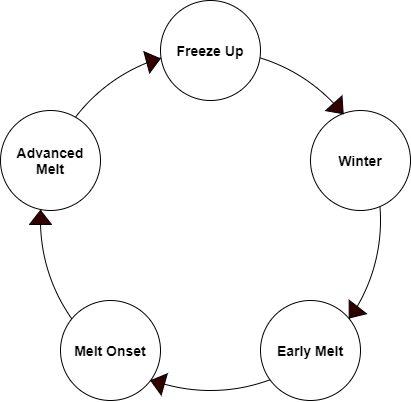
\includegraphics[scale =0.5]{Sea Ice Lifecycle diagram.png}
    \caption{Diagram showing the lifecycle of Antarctic Sea Ice as observed using Microwaves based on the information from \textcite{barber2005microwave}. The cycle begins with the congealing of the ocean surface known as Freeze Up with peak ice formation during Winter, the second half of the cycle is characterised by various stages of melt with complete sea ice retreat occurring in the Summer}
    \label{fig:ice_diag}
\end{figure}

The Southern Ocean plays host to high-cyclonic activity and wave activity which constantly perturb the ice \cite{vichi2019effects}. This results in the formation of a semi-congealed region of ice surrounding the continent. Sea ice in the Southern Ocean follows a unique formation that takes place over a single seasonal cycle. The formation in the Autumn months where the mean sea temperature supercools to $-1.8^{\circ}C$ \cite{womack_2020}. These conditions form the start of the ice cycle known as the "Freeze Up" \cite{barber2005microwave}. During this period, ice crystals begin to form and collect resulting in Frazil Ice \cite{barber2005microwave}. Oceanic waves and strong winds wind cause the frazil ice to mix with the surface layer of the ocean. This results in a slick, shiny layer with a thickness of 0.1 -1 cm called grease ice. The collection of grease and frazil ice is referred to as new ice  \cite{womack_2020} which grows as the average air temperature drops. Eventually, groups of frazil start to congeal into small circular plates known as pancakes \cite{womack_2020} growing between 30cm and 3m in diameter \cite{icedefinition1992}. As the conditions calm down, the plates further congeal and grow in size until an equilibrium is reached\cite{barber2005microwave}. \par 

The winter stage occurs when the sea ice is at the fullest extent. During this period, low temperatures, high precipitation and wide-spread ice coverage result in a layer of snow formed on the new ice floes \cite{sturm2009snow}  Full developed pancakes continue to accumulate new ice and grow into ice floes with diameters ranging from 20m (small floes) to 10km (giant). newly developed floes with a layer of snow are termed first-year ice. Both first-year ice and young ice \footnotetext{Ice floes with a thickness of 10 - 30 cm \cite{icedefinition1992}} account for the majority of ice in the region. Strong winds in the marginal ice zone cause the ice floes to drift over long distances \cite{alberello2019drift}. In areas with strong wind activity and high ice floe density, collisions between floes can occur \cite{Antseaice}. Fractures and breaking occur as a result of these collision resulting in brash ice \cite{icedefinition1992} and additional deformation of the floes through rafting and ridging \cite{icedefinition1992} \cite{womack_2020} \par 

\begin{figure}[H]
    \centering
    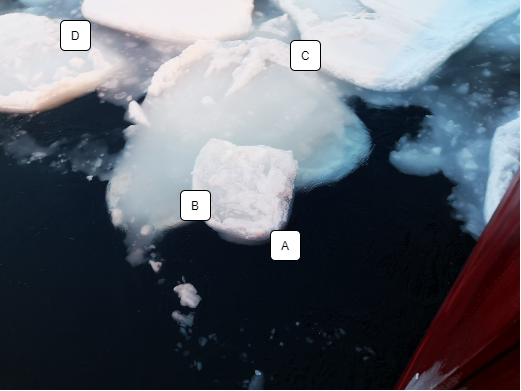
\includegraphics[scale = 0.5]{Ice Floes.png}
    \caption{Diagram showing examples of ice deformation. Constant collisions between ice floe result in ridging (A), or the stacking of ice floes (B) known as rafting. snow (C) typically forms along the ridges which can potentially overload the floe and cause flooding (D). Photo was taken during the SCALE 2019 expedition by the author.}
    \label{fig:ice_deform}
\end{figure}
The final phase of the life cycle begins after the winter period as the air temperature begins to increase. Moisture starts to form in the snow which signifies the beginning of early melt \cite{barber2005microwave}. further warming of the region results in larger pockets of moisture forming in ice eventually resulting in the gradual break down of the ice floe \cite{barber2005microwave}. Melt Onset occurs when the liquid water measured accounts for 7\% \cite{barber2005microwave} of the total mass water pockets (grains) form in the ice floe and begin to increase. Finally, when the snow becomes saturated with water, the ice floe melts and the sea ice layer retreats towards the continent in a phase known as an advanced melt. \cite{barber2005microwave}.

\begin{figure}[H]
    \centering
    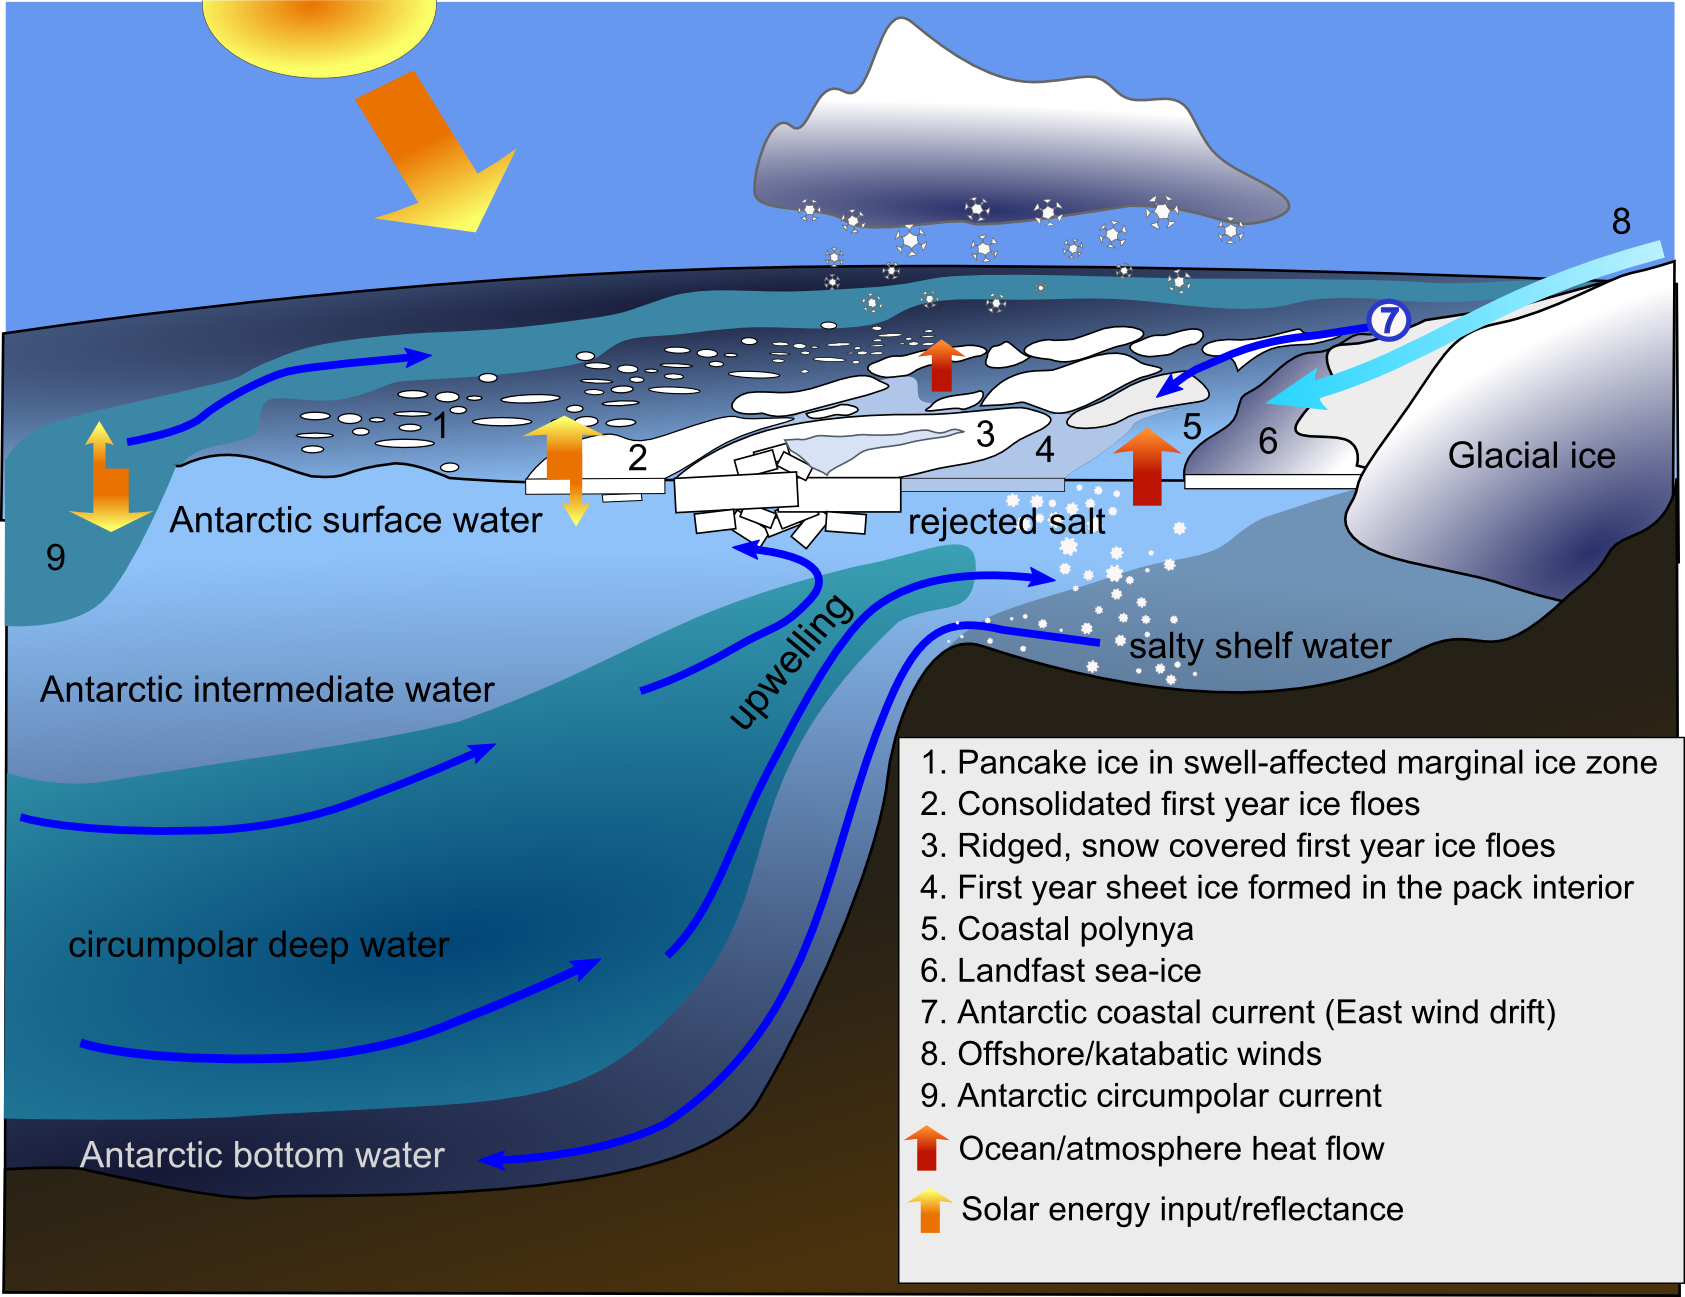
\includegraphics[width = 7cm,height=6cm]{AntDiag.png}
    \caption{Diagram showing the expanse of sea ice in the southern ocean. Packed ice forms closer to the continent in calmer conditions while strong oceanic currents and extreme temperatures result in the formation of semi-consolidated ice in the marginal ice zone (1 - 5). Here, ice formation is highly seasonal expanding to a maximum in winter and retreating to a minimum in summer. Sea ice acts as a boundary layer influencing heat and gaseous exchange between the atmosphere and ocean. Figure is taken from \cite{Antseaice}}
    \label{fig:sea_ice}
\end{figure}

Subsequent Heating and melting stages result in the growth of existing ice floes and the fusing of brash ice and new ice into larger masses \cite{arrigo2004large}. Existing ice floes may come together and fuse along ridges \cite{womack_2020}. Additionally, a redistribution of sea ice occurs where large segments of sea ice are compressed leaving large open water regions \cite{womack_2020}. During this stage, the total sea ice mass remains constant, however, deformation of these ice floes results in changes to the thicknesses. Ice floes that overlap when fusing will be thicker than unperturbed ice floes. Uneven ice thickness results in uneven heat exchange between the ocean-ice-atmosphere which has serious implications in a warming climate \cite{womack_2020}.

\subsection{Effects of snow on sea ice formation}

\begin{figure}[H]
    \centering
    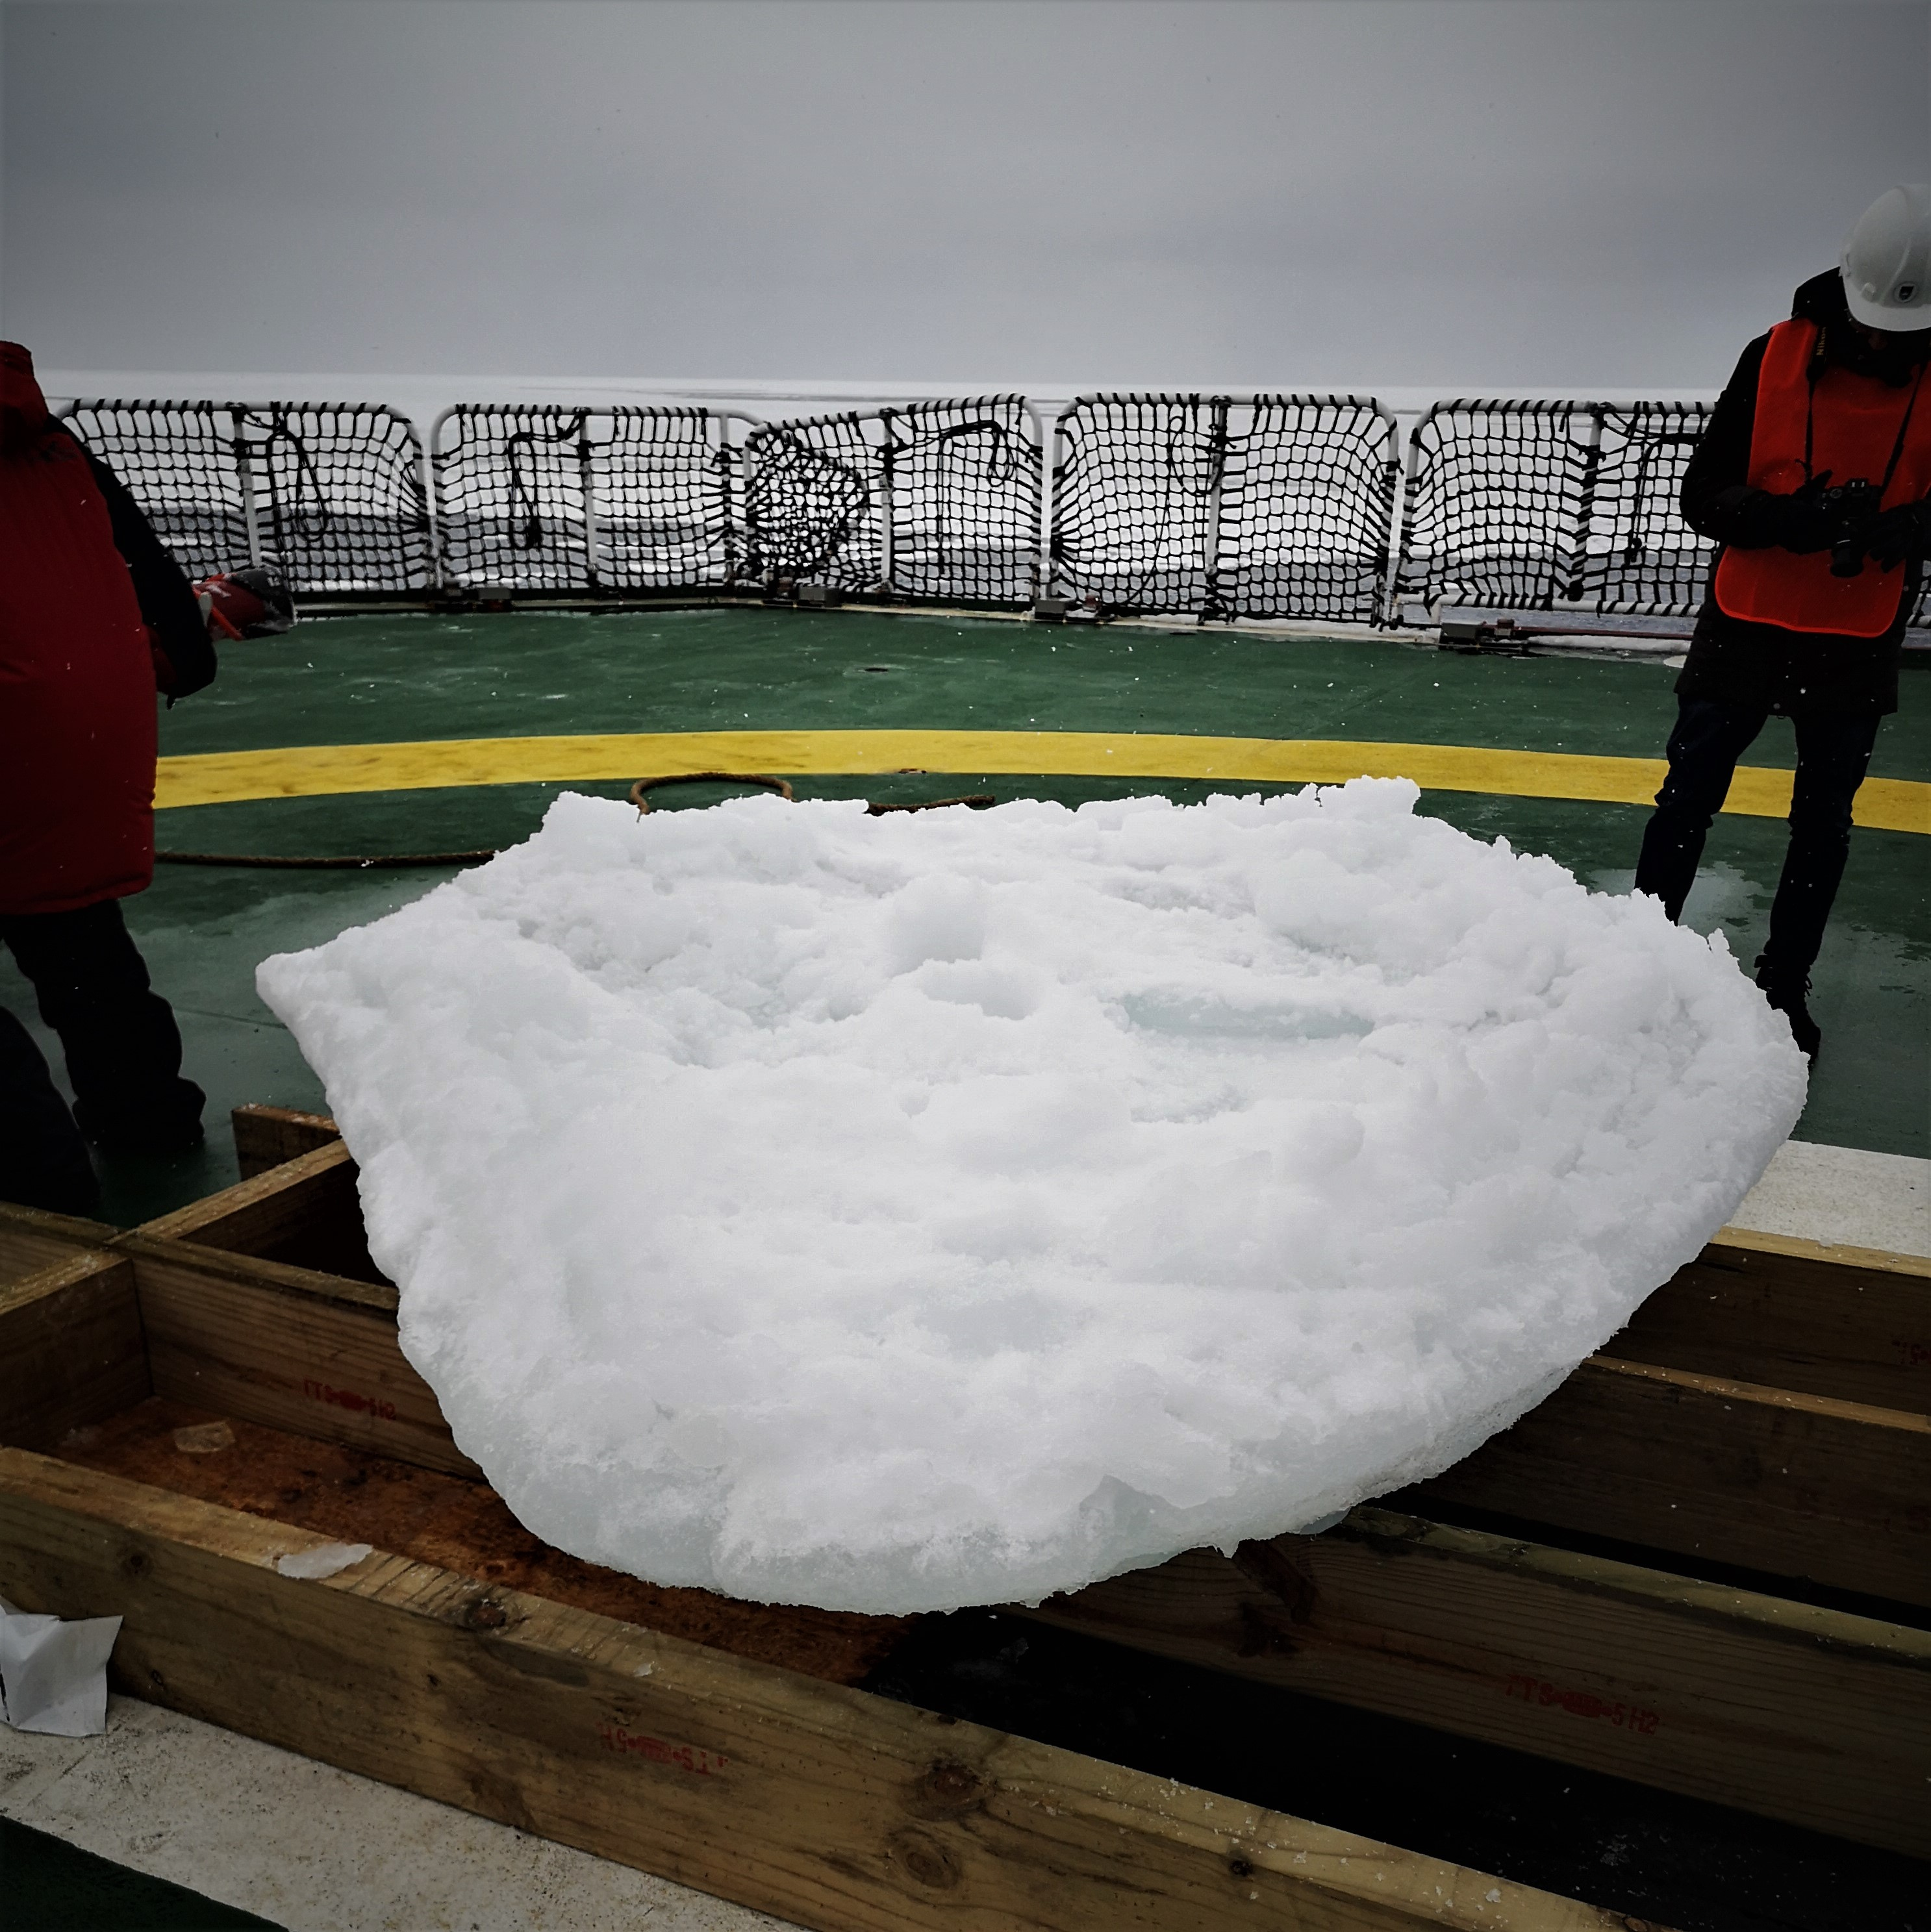
\includegraphics[width = 8cm, height =5cm]{stand alone ice floe.jpg}
    \caption{ Snow growth on a Small Ice floe retrieved from the marginal ice zone during the SCALE 2019 winter expedition. This ice floe is completely covered in snow indicating minimal flooding and no rafting has occurred. The misshapen ridges are indicative of collisions. Photo was taken during the 2019 SCALE winter expedition by the author.}
    \label{fig:lonefloe}
\end{figure}
Snow cover has been shown to significantly impact the physical properties and formation of ice floes \cite{sturm2009snow}. Cold, dry conditions coupled with calm seas and no winds will cause rapid thermodynamic sea ice growth \cite{sturm2009snow} resulting in dry, low salinity snow forming on the surface of existing sea ice floes. However, In damp, turbulent conditions, sea ice growth occurs much slower \cite{sturm2009snow} resulting in wet snow forming on newer ice floes. Hence, snow can be used as an indicator of the formation conditions surrounding the ice floes \cite{sturm2009snow}. Snow typically grows along the ridges of Antarctic sea ice  \cite{massom2001snow} and can grow up to 1m in height \cite{barber2005microwave}. Snow has a higher albedo exchange than sea ice thereby significantly impacting the short-wave energy exchange with the atmosphere and ocean \cite{massom2001snow} and slowing down the rate of heat exchange. Additionally, this thermodynamic interaction forms the ice-albedo feedback mechanism \cite{MASSOM2010149} which regulates the growth and coverage of sea ice. Additionally, snow provides a source of freshwater which affects the salinity and insulates the sea ice against the sun's UV rays thereby maintaining the optical appearance of the ice \cite{MASSOM2010149}. Snow cover plays a pivotal role in the sea ice growth cycle as snow growth of at-least 10cm \cite{galin2012measuring} significantly reduces the melting of an ice flow. However, the consequence of such growth is the thermal insulation stunts the ice floe development \cite{galin2012measuring}. Significant growth of snow can depress the ice floe below the waterline resulting in the snow freezing and forming snow ice \cite{icedefinition1992} \cite{galin2012measuring}.

\begin{figure}[H]
    \centering
    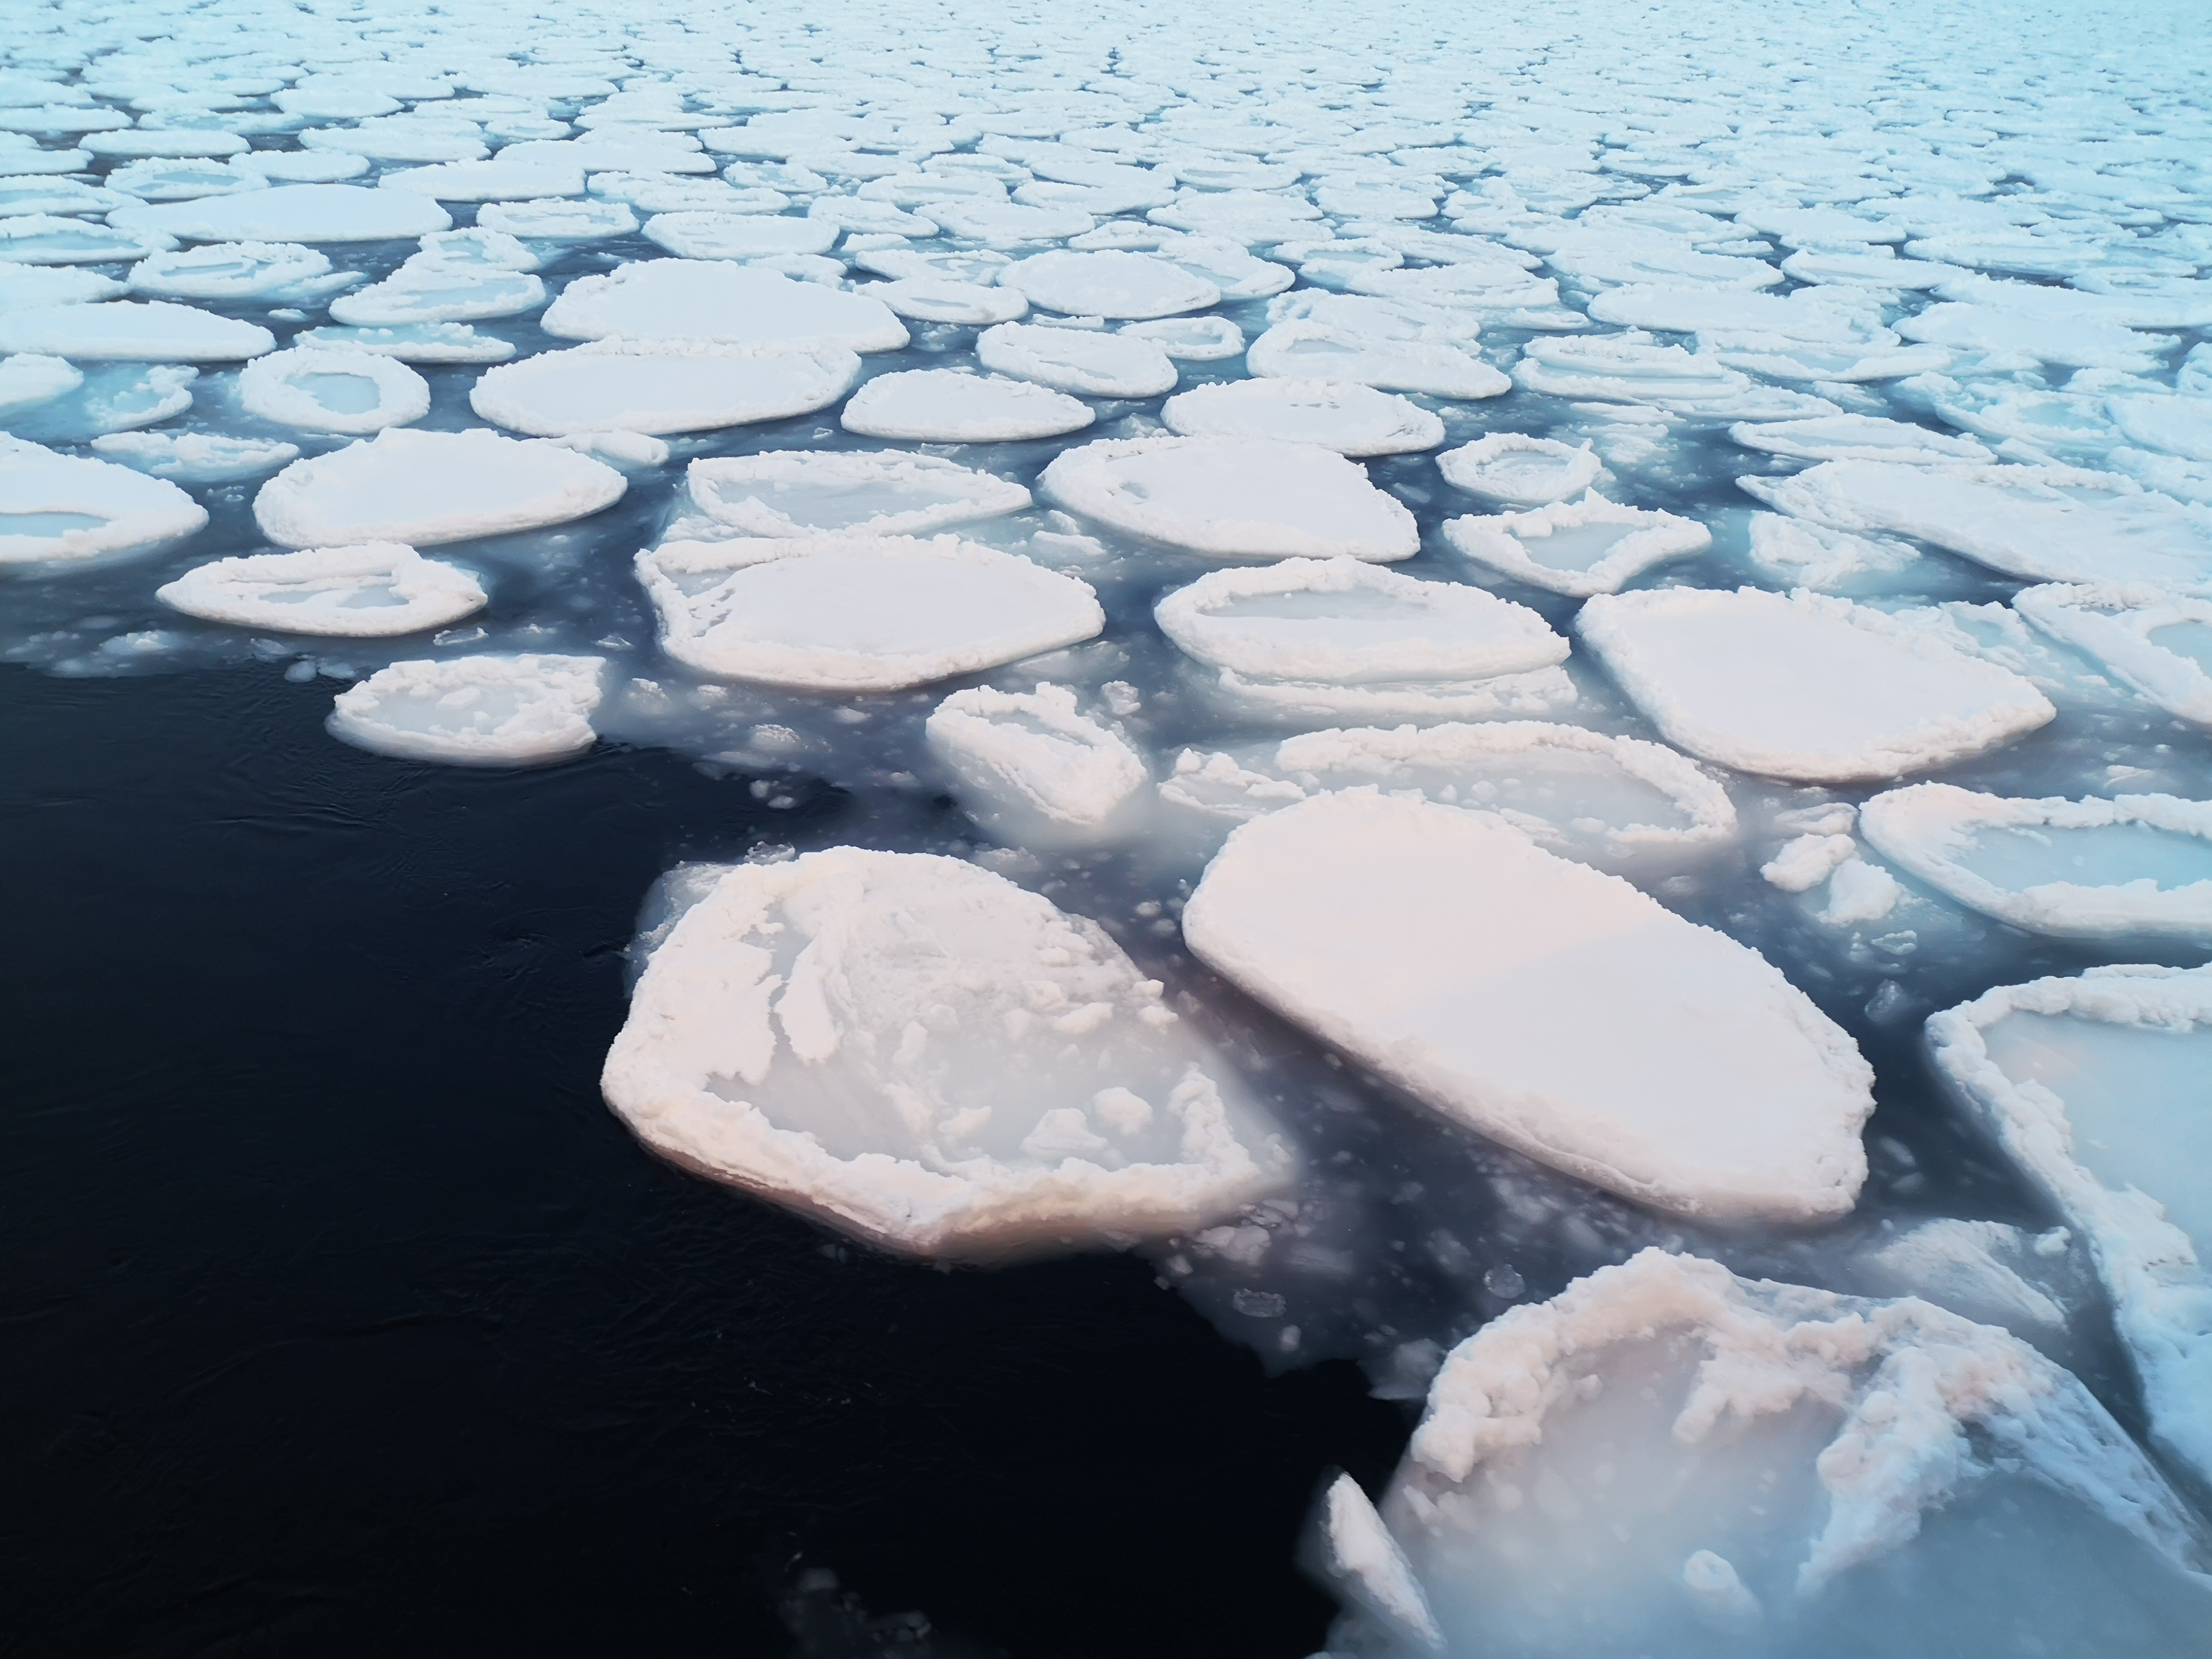
\includegraphics[width = 10cm, height = 8cm]{floe snow.jpg}
    \caption{Ice floes in the marginal ice zone exhibiting snow growth. Ice growth is more prominent along the ridges while some of the floes exhibit flooding. Photo taken during SCALE 2019 winter expedition by the author.}
    \label{fig:ridging}
\end{figure}

\subsection{Numerical modeling of polar stochastic processes}

In this section, modelling techniques for the polar region are explored. Here, the focus is given on developing models for Polar sea ice mechanics and dynamics. An overview of these models is given along with a description of the variables as well as the scope of each model.

\subsubsection{Numerical Modeling of Sea Ice}

The Hibler model is a numerical designed to investigate sea ice dynamics and thermodynamics in the Arctic region \cite{hibler1979dynamic}. This model attempts to couple the sea ice dynamics to Sea ice thickness and uses this relationship to investigate the relationship between the effects of sea ice and the climate. Work so far has largely studied these effects independently using factors that largely ignore the inherent mechanical properties of Sea Ice \cite{hibler1979dynamic}. Coupling these effects would allow for a more general descriptor of Sea Ice spread regions.\par

The model is based off \textcite{coon1974modeling} AIDJEX \cite{hibler1979dynamic}, who use plastic-elastic constitutive laws to describe large-scale sea Ice spreads. It is assumed that cracks, ridges, and leads are randomly distributed on large scales \footnote{100 km from \textcite{coon2007arctic}}. While the Hibler model is not as complex, it is more robust as it allows for larger time-steps and simplifies system boundaries. Here, sea ice is modelled using similar viscous plastic laws \cite{hibler1979dynamic} that allow for non-linear plastic flows to be modelled without severe limitations by large time-steps. The model uses the following components:

\begin{enumerate}
     \item    Momentum balance  - air and water stress
     \item    Coriolis force
     \item    Inertial forces
     \item    Constitutive laws - ice stress, strain, strength
     \item    Ice thickness distribution - accounting for open water patches, changes in thickness and Concentration
     \item    Ice strength 
\end{enumerate}
\begin{equation}
\frac{mDu}{Dt} = -mfk\times u +\tau_a +\tau_w -mg \nabla H +F 
\end{equation}

$\frac{D}{Dt}$ is the substantial time derivative, k is a unit vector, u is the sea ice velocity, m is the ice mass and f is the Coriolis parameter. Forces in the equation $\tau_a$, $\tau_w$ represent the stress of the air and water respectively where F is the force related to the internal ice stresses. H is the sea surface dynamic height and g is the acceleration due to gravity. Assuming constant turning angles, The air and water momentum equations are as follows
\begin{equation}
    \tau_a = \rho_a C_a|U_g|(U_g cos(\phi)+k\times U_g sin(\phi))
\end{equation}

\begin{equation}
    \tau_w = \rho_w C_w|U_w-u|[(U_w-u)cos(\phi)+k\times(U_w-u)sin(\phi)]
\end{equation}


where $\rho_a $ and $\rho_w$ are the densities of air and water, $C_a$/$C_w$ are the drag coefficients, $U_g$ is the geostrophic wind and $U_w$ is the geostrophic ocean current\par

The Hibler model is the de facto numerical model for large scale ice process \cite{Rutgher2019SmallScale}. The model is used to describe an area of 10 - 100km$^2$, Small scale models are still in development \cite{Rutgher2019SmallScale}.\par 

\subsubsection{Numerical Modeling of Ocean Waves}
Ocean waves are comprised of multiple spectral components with different magnitudes and wave periods knowledge of these spectral components is important for understanding the wave attenuation model \cite{williams2013wave} where, assuming the ice is modelled as a viscous fluid, wave energy is exponentially attenuated \cite{meylan2014situ}\cite{williams2013wave} with distance travelled into the ice due to partial reflections with the ice floes. The rate of attenuation is dependant on the wavelength however an exact mathematical relationship has not been found. The major issue with verifying these models is the lack of robust data availability \cite{meylan2014situ} thereby reaffirming the need for in-situ measurements.\par 
%%% TODO: INCLUDE WILLIAMS WAVE MODELS AND EQUATIONS FOR WAVE SPECTRUM ANALYSIS
\textcite{williams2013wave} describe three fundamental components of Waves in Ice Modeling. These are advection, attenuation, and ice breakage \cite{williams2013wave}. Advection and Attenuation describe how energy transfer occurs between waves and ice and are dependant on the group velocity $c_g$ and the attenuation factor $\hat{\alpha}$ which, in turn, are dependant on the frequency of the wave \cite{williams2013wave}. Also, the properties of ice are significant. These include Young's modulus $Y$, Poisson Ratio $\nu$, strain $\epsilon$ and viscous damping parameter $\Gamma$. The initial Floe Size Distribution and sea ice concentration are also considered. The assumption is that wave breakage feeds back into the model with a new Floe Size distribution \cite{williams2013wave}. \par

Wave advection is described by the following energy model:
\begin{equation}
    \frac{1}{c_g}(\partial_t +c_g\partial_x)S(\omega;x,t) = R_{in}- R_{ice} - R_{other}- R_{nl}
\end{equation}
where $R_{in}$ is the wind input energy, $R_{ice}$,$R_{nl}$,$R_{other}$ represent the energy loss from ice, other sources as well as non linear energy exchanges. $S(\omega;x,t)$ represents the waves in terms of its energy spectral density \cite{williams2013wave} For this model, the energy input is considered to come only from the Rate of exchange between ocean and Ice. Hence all other energy rates are considered 0 and $R_{ice}$ is defined in terms of $\hat{alpha} \text{ and } S$
\begin{equation}
   \frac{1}{c_g}(\partial_t +c_g\partial_x)S(\omega;x,t)  = -\hat{\alpha}(\omega,c,h,\langle D \rangle)S(\omega;x,t)
\end{equation}

$\hat{\alpha} = \frac{\alpha}{\langle D \rangle}$ describes the average attenuation per ice floe. In terms of Ice thickness and wave period \cite{williams2013wave}. By this definition, $R_ice$ is quasi linear \cite{williams2013wave} since a wave with a significantly large Energy spectral density can break the floe decreasing the dimensions $\langle D \rangle$ and increase the dimensional attenuation factor $\hat{\alpha}$. The  operator $(\partial_t +c_g\partial_x)$ serves as the lagrangian reference fram at a moving velocity $c_g$. Finally, by breaking the above model into:
\begin{subequations}
\begin{align}
    \frac{dx}{dt} = c_g(\omega,t_*,x) \label{advect}\\
    \frac{dS(\omega;x,t)}{dx} = -\hat{\alpha}(\omega,x,t_*,S_*)S(\omega;x,t) \label{atten}
\end{align}
\end{subequations}

we can describe the dynamics of the sea ice during a breaking event at a time $t_*$ \cite{williams2013wave}. Hence, the model is broken up into an advection model in \ref{advect} and an attenuation model in \ref{atten}.\par

The next step in the model is determining the mathematical model for wave energy. A stochastic approach is taken to define key wave parameters \cite{williams2013wave}. The Significant wave height is found using the formula
\begin{equation}
    H_s = 4\sqrt{m_0[n]}
\end{equation}
$m_n[\eta]$ describes the mean square surface sea elevation of a particle and is derived from the Spectral Density $S$ \cite{williams2013wave}.
\begin{equation}
    m_n[\eta] = \int_{0}{\infty}S(\omega)\omega^nd\omega
\end{equation}

The significant wave height can be considered 4 times the standard deviation of the surface elevation \cite{meylan2014situ}. finally, by determining the significant wave height, the dominant wave period can be calculated as $\frac{1}{f_d}$ where $f_d$ is the frequency at which the dominant wave period occurs \cite{meylan2014situ}.
\newpage
\section{In-situ climate sensing technologies}
\label{ch2:secdevice}
\begin{figure}[H]
    \centering
        \begin{subfigure}[b]{0.24\textwidth}
         \centering
         \begin{tikzpicture}
             \node[anchor=south west,inner sep=0] (image) at (0,0) { 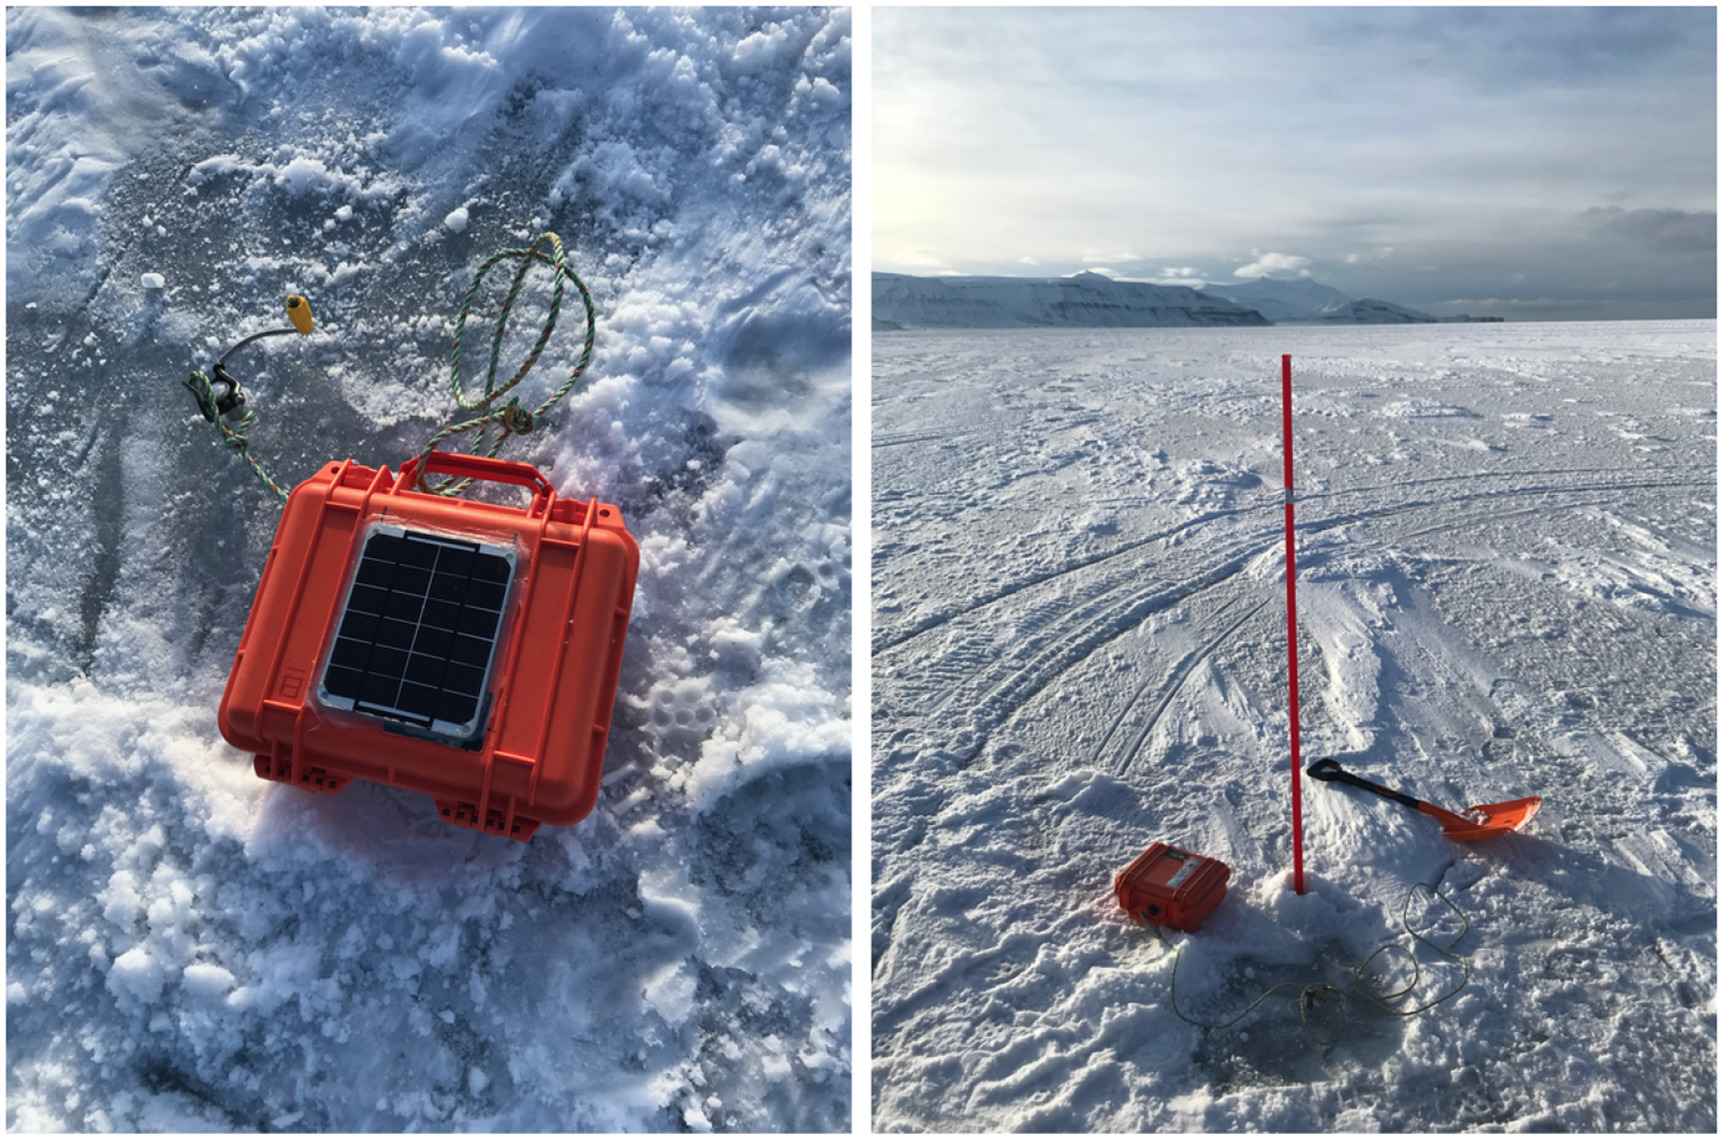
\includegraphics[width = 4cm,height=4cm]{WIIB.jpg}};
    \begin{scope}[x={(image.south east)},y={(image.north west)}]
        \draw[color=black, ultra thin,fill=white] (0.0,0.0) rectangle (0.21,0.16) node[pos=.5] {A};
    \end{scope}
    \end{tikzpicture}
         \label{fig:WIIB}
     \end{subfigure}%
     \hfill
        \begin{subfigure}[b]{0.24\textwidth}
         \centering
        \begin{tikzpicture}
             \node[anchor=south west,inner sep=0] (image) at (0,0) { 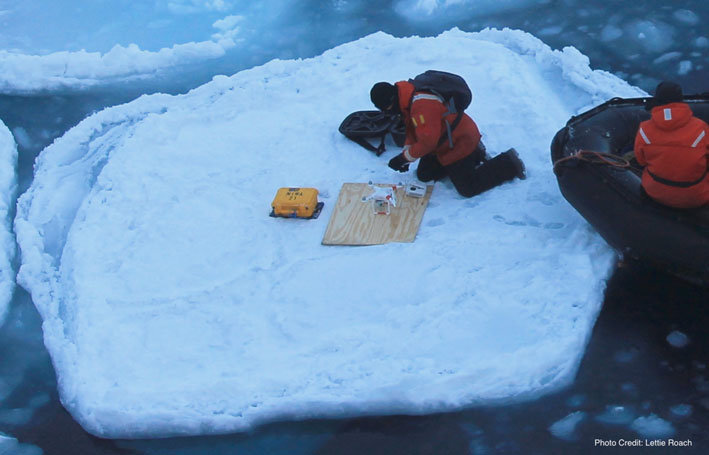
\includegraphics[width = 4cm,height=4cm]{WIIOS.png}};
    \begin{scope}[x={(image.south east)},y={(image.north west)}]
        \draw[color=black, ultra thin,fill=white] (0.0,0.0) rectangle (0.21,0.16) node[pos=.5] {B};
    \end{scope}
    \end{tikzpicture}
         \label{fig:WIIOS}
     \end{subfigure}%
     \hfill
    \begin{subfigure}[b]{0.24\textwidth}
         \centering
                  \begin{tikzpicture}
             \node[anchor=south west,inner sep=0] (image) at (0,0) { 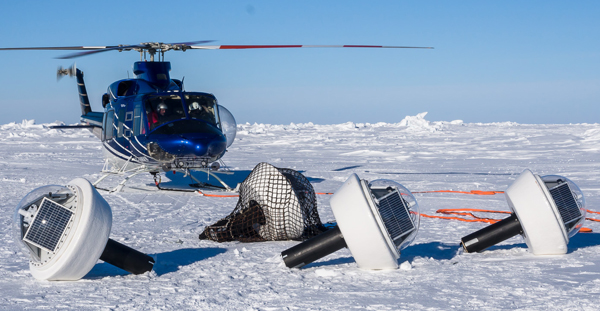
\includegraphics[width = 4cm,height=4cm]{doble.jpg}};
    \begin{scope}[x={(image.south east)},y={(image.north west)}]
        \draw[color=black, ultra thin,fill=white] (0.0,0.0) rectangle (0.21,0.16) node[pos=.5] {C};
    \end{scope}
    \end{tikzpicture}
         \label{fig:NDWB}
     \end{subfigure}%
     \hfill
    \begin{subfigure}[b]{0.24\textwidth}
         \centering
                  \begin{tikzpicture}
             \node[anchor=south west,inner sep=0] (image) at (0,0) { 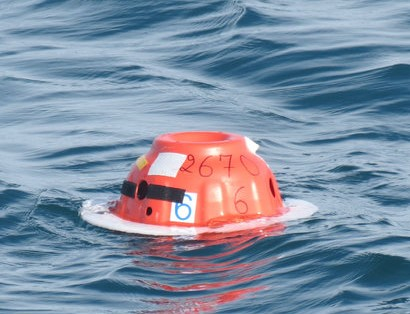
\includegraphics[width = 4cm,height=4cm]{SKIB.png}};
    \begin{scope}[x={(image.south east)},y={(image.north west)}]
        \draw[color=black, ultra thin,fill=white] (0.0,0.0) rectangle (0.21,0.16) node[pos=.5] {D};
    \end{scope}
    \end{tikzpicture}
         \label{fig:SKIB}
     \end{subfigure}%
     \hfill
     \begin{subfigure}[b]{0.24\textwidth}
         \centering
                  \begin{tikzpicture}
             \node[anchor=south west,inner sep=0] (image) at (0,0) { 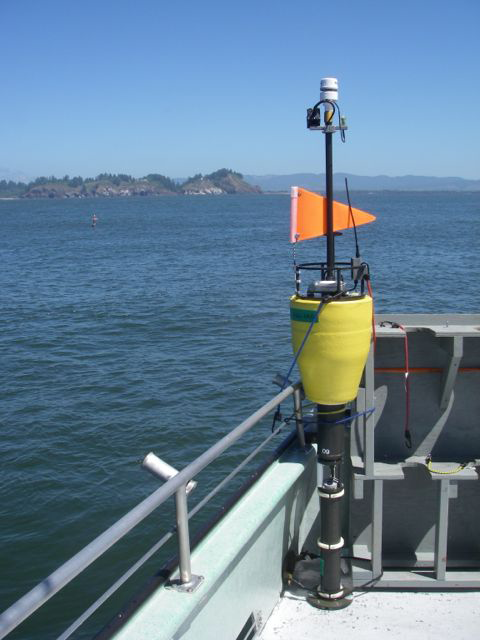
\includegraphics[width = 4cm,height=4cm]{swift_4.png}};
    \begin{scope}[x={(image.south east)},y={(image.north west)}]
        \draw[color=black, ultra thin,fill=white] (0.0,0.0) rectangle (0.21,0.16) node[pos=.5] {E};
    \end{scope}
    \end{tikzpicture}
         \label{fig:SWIFT}
    \end{subfigure}%
    \hfill
    \begin{subfigure}[b]{0.24\textwidth}
         \centering
                  \begin{tikzpicture}
             \node[anchor=south west,inner sep=0] (image) at (0,0) { 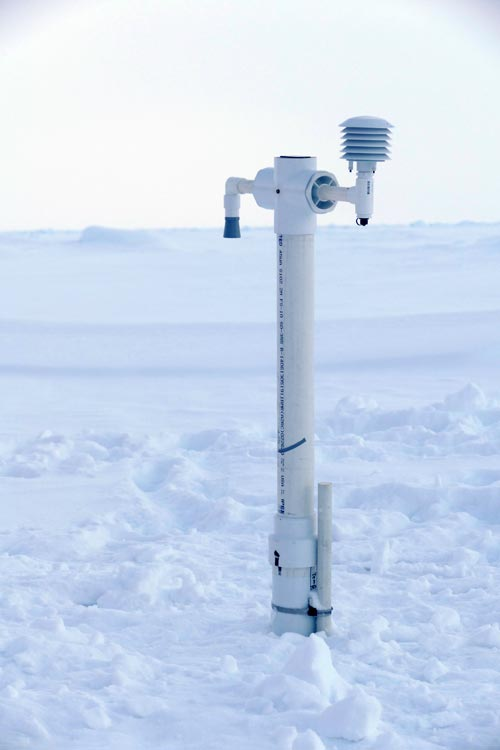
\includegraphics[width = 4cm,height=4cm]{SIMB.jpg}};
    \begin{scope}[x={(image.south east)},y={(image.north west)}]
        \draw[color=black, ultra thin,fill=white] (0.0,0.0) rectangle (0.21,0.16) node[pos=.5] {F};
    \end{scope}
    \end{tikzpicture}
    \label{fig:SIMB}
    \end{subfigure}%
    \hfill
    \begin{subfigure}[b]{0.24\textwidth}
         \centering
                  \begin{tikzpicture}
             \node[anchor=south west,inner sep=0] (image) at (0,0) { 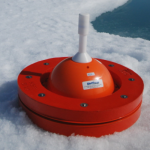
\includegraphics[width = 4cm,height=4cm]{UptempO.png}};
    \begin{scope}[x={(image.south east)},y={(image.north west)}]
        \draw[color=black, ultra thin,fill=white] (0.0,0.0) rectangle (0.21,0.16) node[pos=.5] {G};
    \end{scope}
    \end{tikzpicture}
         \label{fig:UptempO}
    \end{subfigure}%
    \hfill
    \begin{subfigure}[b]{0.24\textwidth}
         \centering
                  \begin{tikzpicture}
             \node[anchor=south west,inner sep=0] (image) at (0,0) { 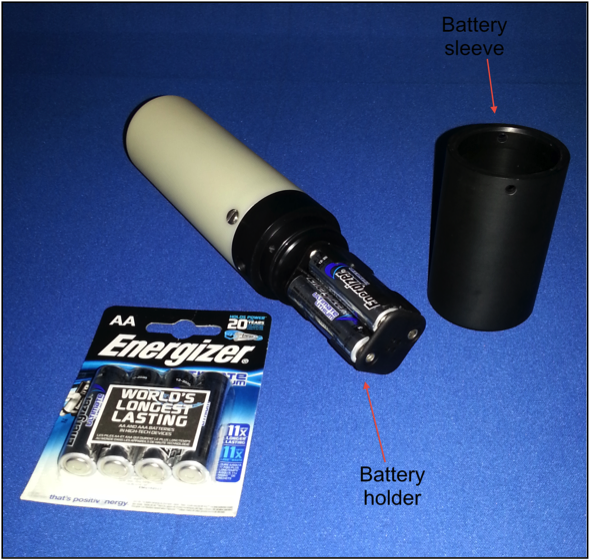
\includegraphics[width = 4cm,height=4cm]{trident.png}};
    \begin{scope}[x={(image.south east)},y={(image.north west)}]
        \draw[color=black, ultra thin,fill=white] (0.0,0.0) rectangle (0.21,0.16) node[pos=.5] {H};
    \end{scope}
    \end{tikzpicture}
         \label{fig:trident}
    \end{subfigure}%
    \hfill
    \caption{ Devices used for the comparison study. Each device has been selected for its notability in published work as well as prevalence in sea ice and wave interactions in the Marginal Ice Zones.Devices are: Wave in Ice Buoy (A) developed by \textcite{rabault2017measurements} (image source: \cite{rabault2017measurements}), Wave in Ice Observational System by \textcite{kohout2015device} (B) (image source: \cite{kohout2020observation}), Novel Wave Directional buoys  (C) by \textcite{doble2017robust} (image source: \cite{doble_wave_2015}), Surface Kinematic buoy (D) by \textcite{guimaraes2018surface} (image source: \cite{guimaraes2018surface}),  Surface Wave Instrument Float Tracking buoy (E) by \textcite{thomson2012wave} (iamge source: \cite{jim_swift_2012}), Seasonal Ice Mass Balance buoy (F) by \textcite{polashenski2011seasonal} (image source: \cite{simbpic}), Polar ISVP (G) by MetOcean (image source: \cite{uptempo}), Trident buoy (H) by Trident (image source: \cite{trident})}
    \label{fig:buoys}
\end{figure}

Autonomous instrumentation has seen increased use for in-situ observations \cite{kennicutt2016delivering}. These devices have typically developed by the commercial sector  \cite{rabault2017measurements}  from companies such as Trident, MetOcean, Seabird and Sea Technology Services (STS). Additionally, academic institutions have also developed in-situ measurement devices such as The University of Washington's SWIFT buoy \cite{thomson2012wave} or University of Dartmouth's Seasonal Ice Mass Balance (SIMB) buoy \cite{polashenski2011seasonal}. While these technologies have the benefit of reliability. They are often expensive \cite{rabault2017measurements} and inflexible to the demands of Polar Science. Technology has reached a point where low-cost alternatives (i.e. off the shelf ) are well documented and reliable enough to be integrated into customized technological solutions as "open source" \cite{rabault2019open}. This term is commonly used for software and hardware that has been licensed for distribution and integration into other projects \cite{bonvoisin2017source}. Open-source software has become more prevalent with the rise of the internet \cite{bonvoisin2017source}. Open-source hardware cannot be directly shared however, the designs are made publicly available to be studied, modified, distributed or shared \cite{bonvoisin2017source}.\par 

The devices are easier to use and could reduce redundancy of devices as well as development/ procurement times. It has also been found that conductor electronics have proven to operate in low temperatures with few problems \cite{rabault2017measurements}. In this section, a comparison of data collection devices is presented with their methodologies as well as effects on the results. Where possible, certain specifications have been converted into standardized formats. To ensure a fair evaluation, data were collected from the latest technical publication of each platform where possible. These publications may not contain all relevant data. In this case, the data entry has been marked with a "Not reported" or "NR". figure \ref{fig:buoys} below shows the devices selected for the comparison.


Eight platforms were selected for the comparison with each device designed by a private company or an institution. The key collaborators as well as the name of the institution are provided in table \ref{tab:device_list}. Where a buoy name is not given, the device will be named after the key contributor to the project. These systems have been selected due to their prevalence in global polar/ oceanographic science as well as notability in publications.

\subsection{Remote Communication}

Table \ref{tab:device_transmissionstrategies} shows that all devices that have been deployed in both the Arctic and Antarctic Marginal Ice Zones use Iridium for remote Telemetry Data.  Other systems such as Zigbee \cite{guimaraes2018surface} are alluded to however these systems are only used when the device is close by. Notably, The SIMB buoy details consideration for Remote communication using the ARGOS satellite network however, the unreliability of the network resulted in irregular timestamped data \cite{planck2019evolution}. The network service, modem and transmission strategy of each device is shown in table \ref{tab:device_transmissionstrategies}.

\begin{figure}[H]
    \centering
    \begin{subfigure}[b]{0.3\textwidth}
    \begin{tikzpicture}
    \node[anchor=south west,inner sep=0] (image) at (0,0) { 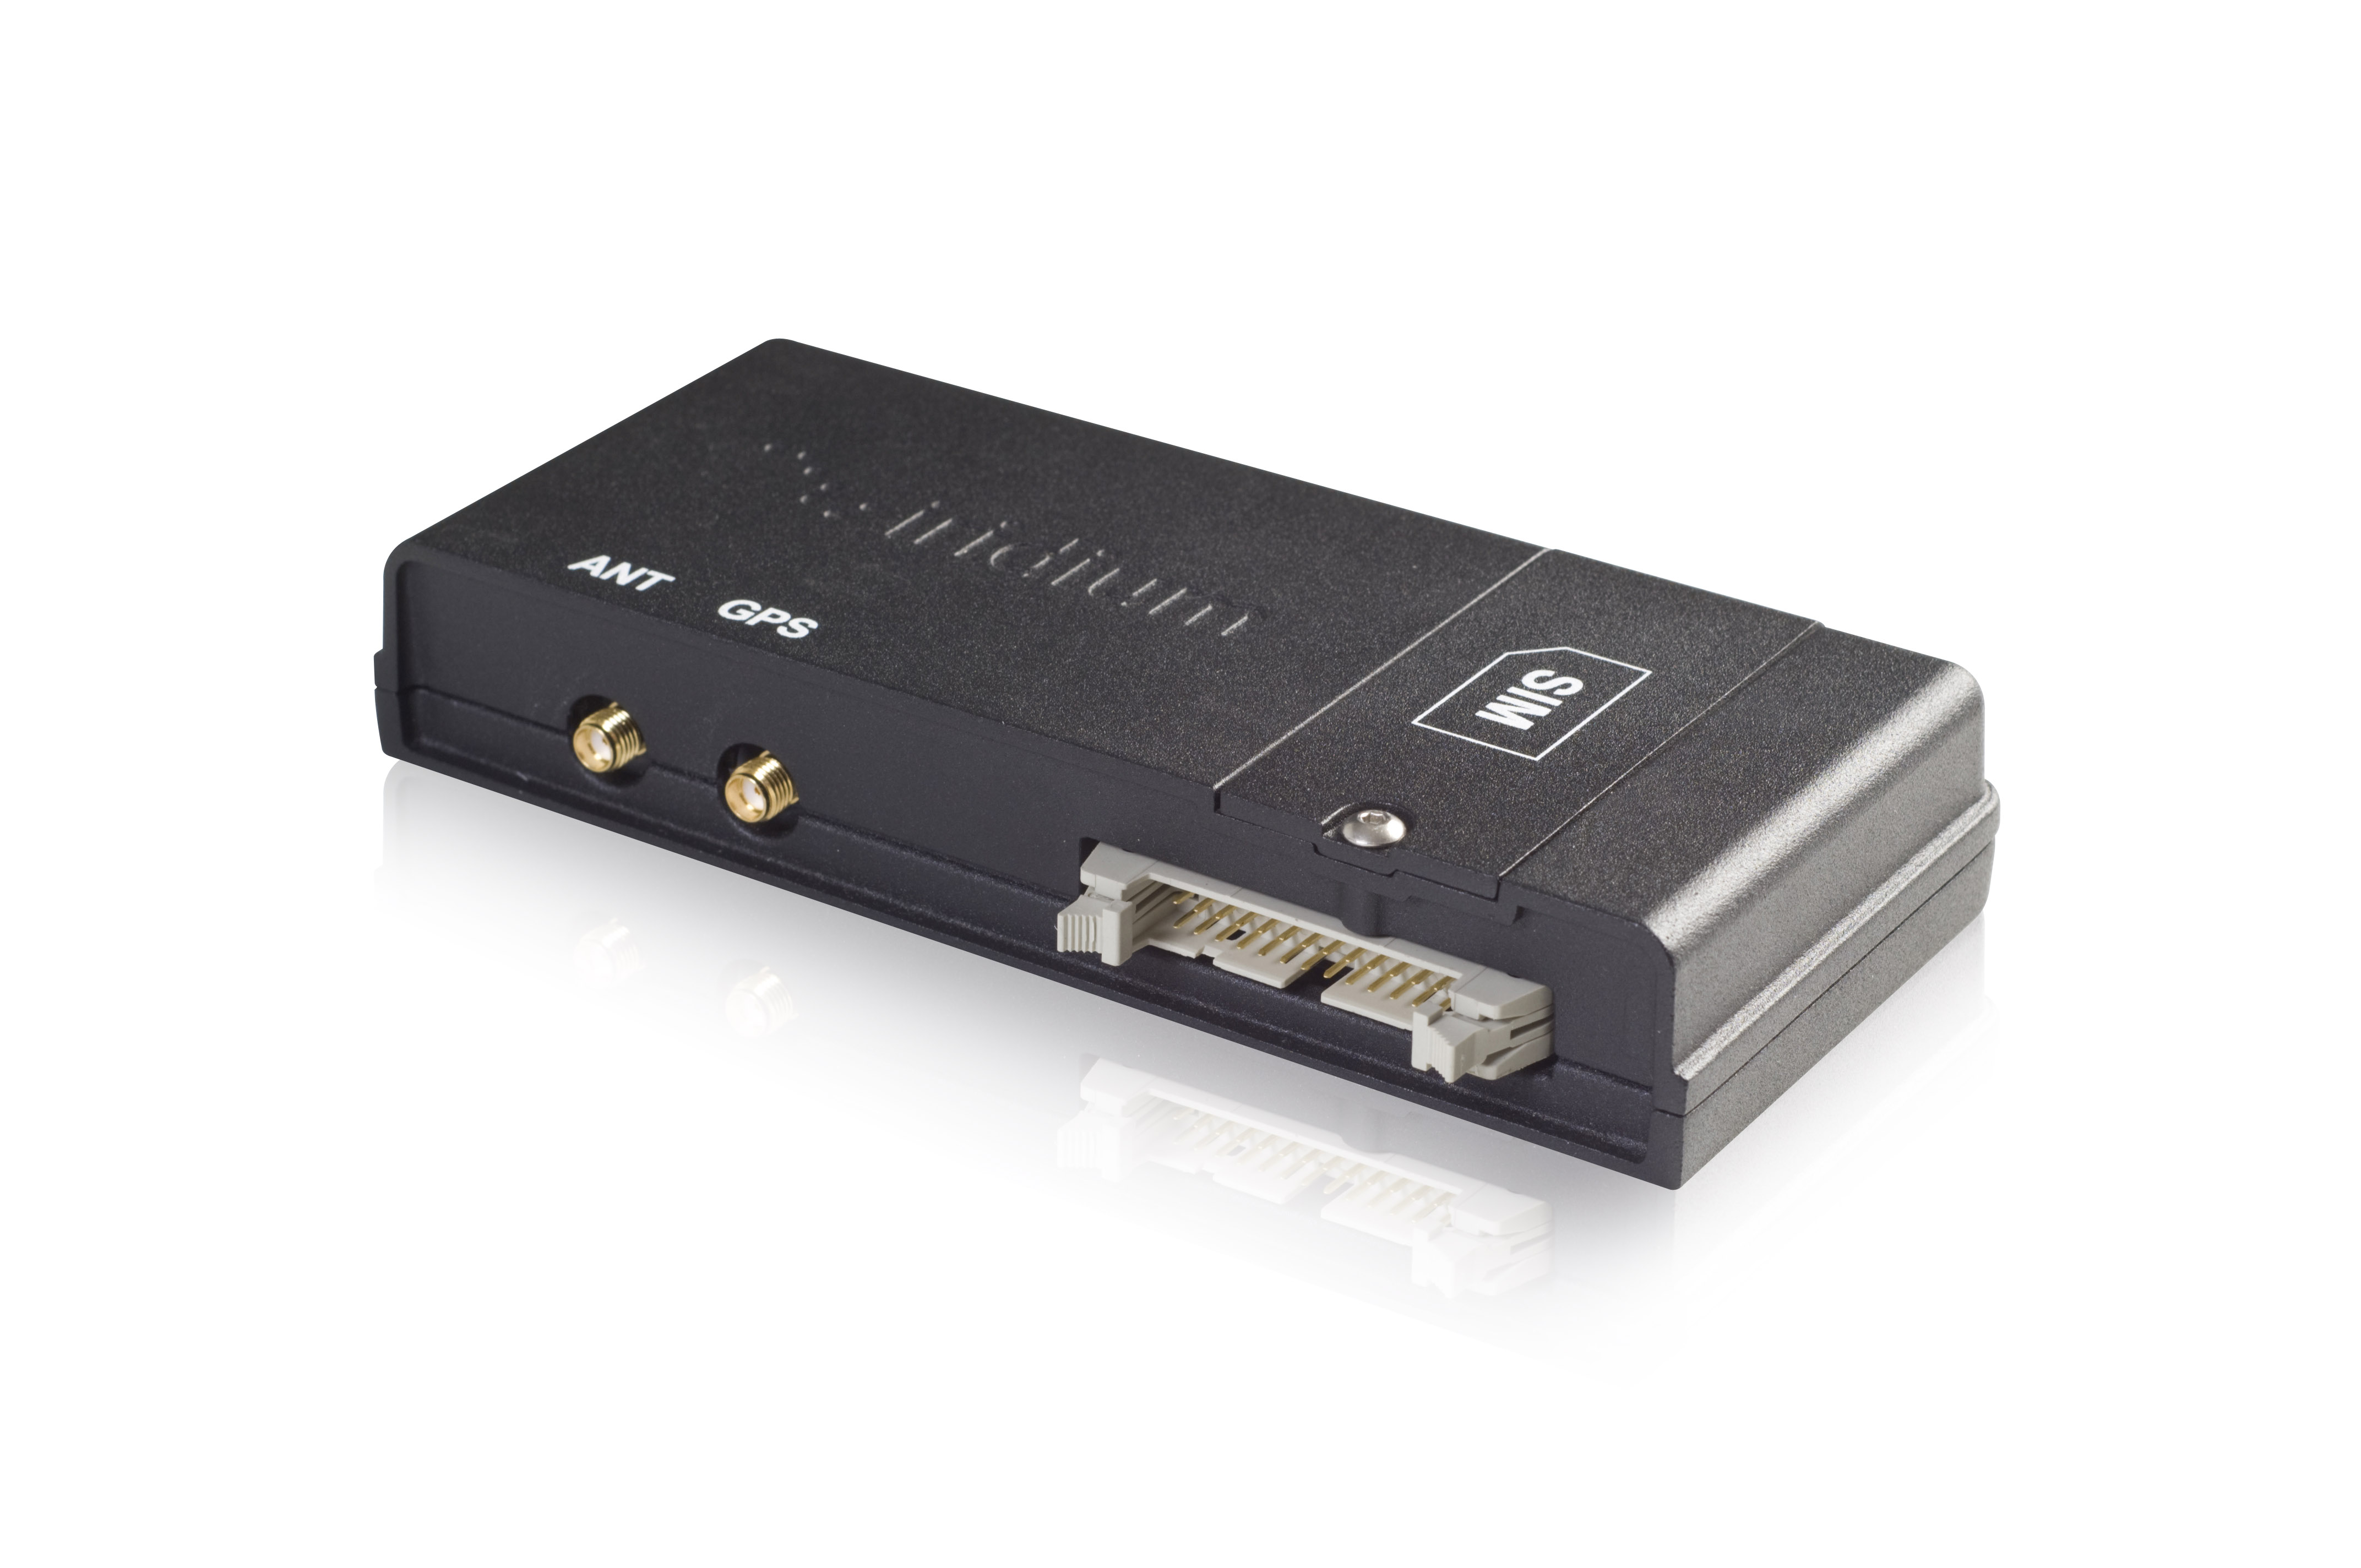
\includegraphics[width = 3cm,height=3cm]{9522B.png}};
    \begin{scope}[x={(image.south east)},y={(image.north west)}]
        \draw[color=black, ultra thin,fill=white] (0.0,0.0) rectangle (0.21,0.16) node[pos=.5] {A};
    \end{scope}
    \end{tikzpicture}
    \end{subfigure}%
    \hfill
        \begin{subfigure}[b]{0.3\textwidth}
            \begin{tikzpicture}
    \node[anchor=south west,inner sep=0] (image) at (0,0) { 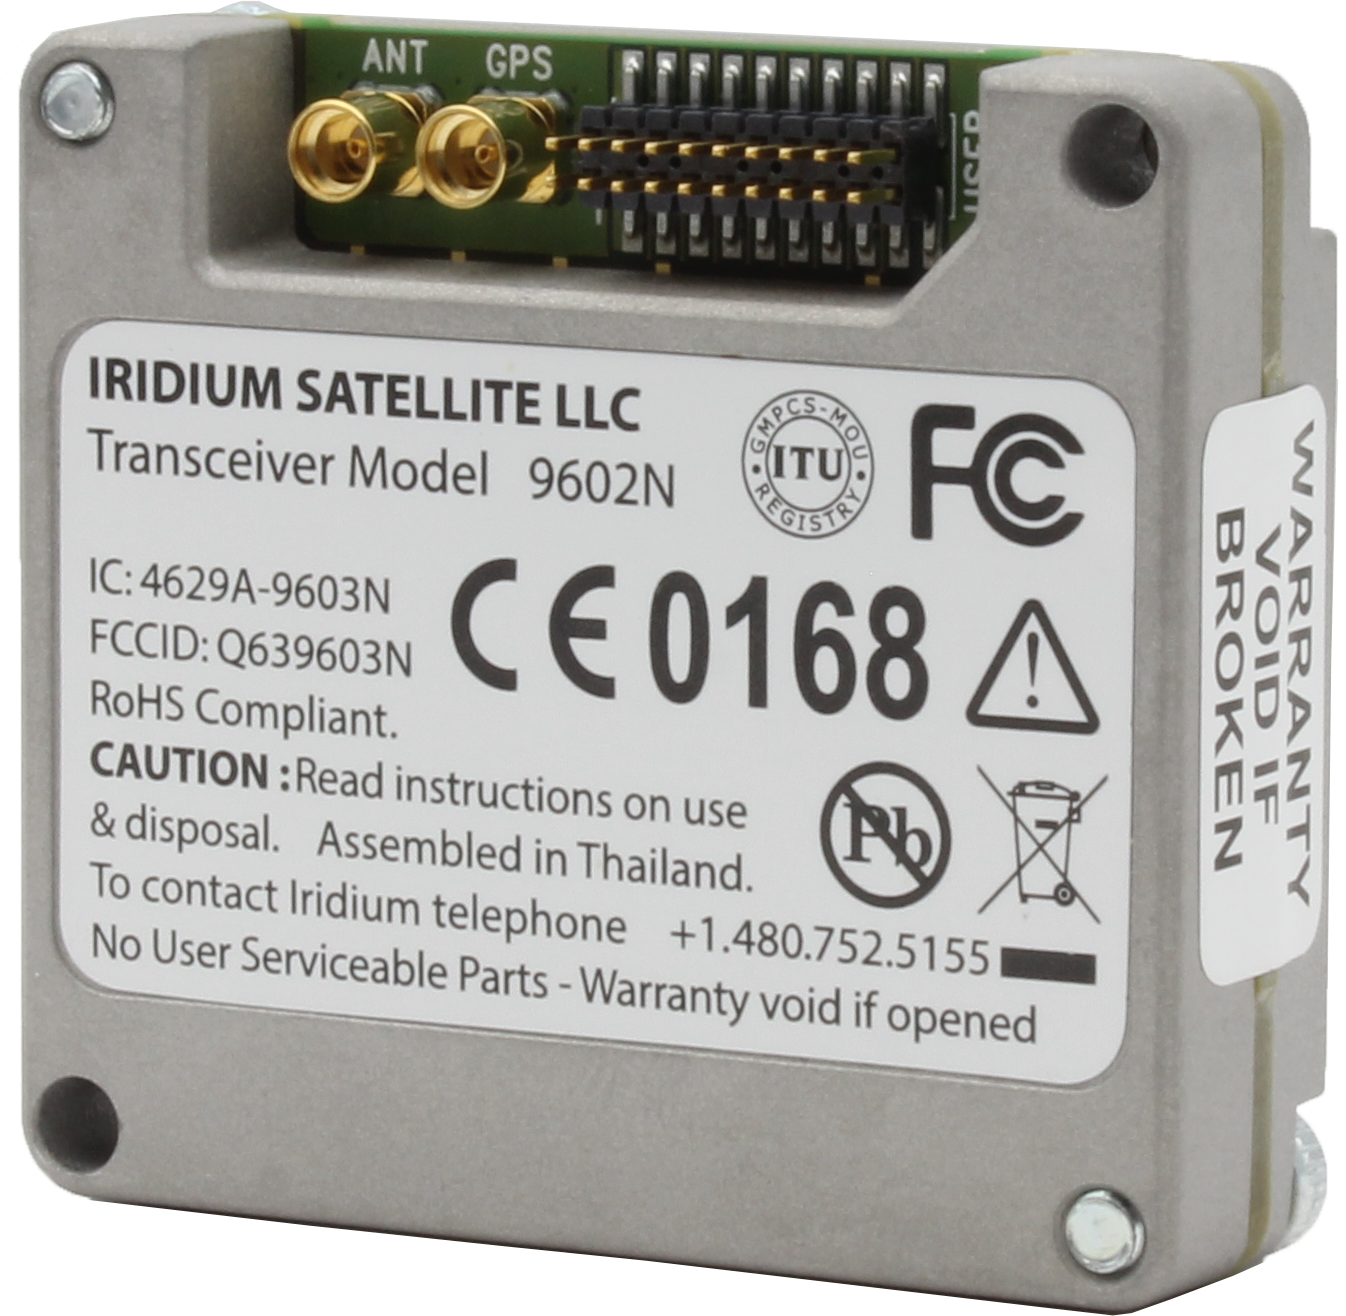
\includegraphics[width = 3cm,height=3cm]{9602.png}};
    \begin{scope}[x={(image.south east)},y={(image.north west)}]
        \draw[color=black, ultra thin,fill=white] (0.0,0.0) rectangle (0.21,0.16) node[pos=.5] {B};
    \end{scope}
    \end{tikzpicture}
    \end{subfigure}%
    \hfill
        \begin{subfigure}[b]{0.3\textwidth}
            \begin{tikzpicture}
    \node[anchor=south west,inner sep=0] (image) at (0,0) { 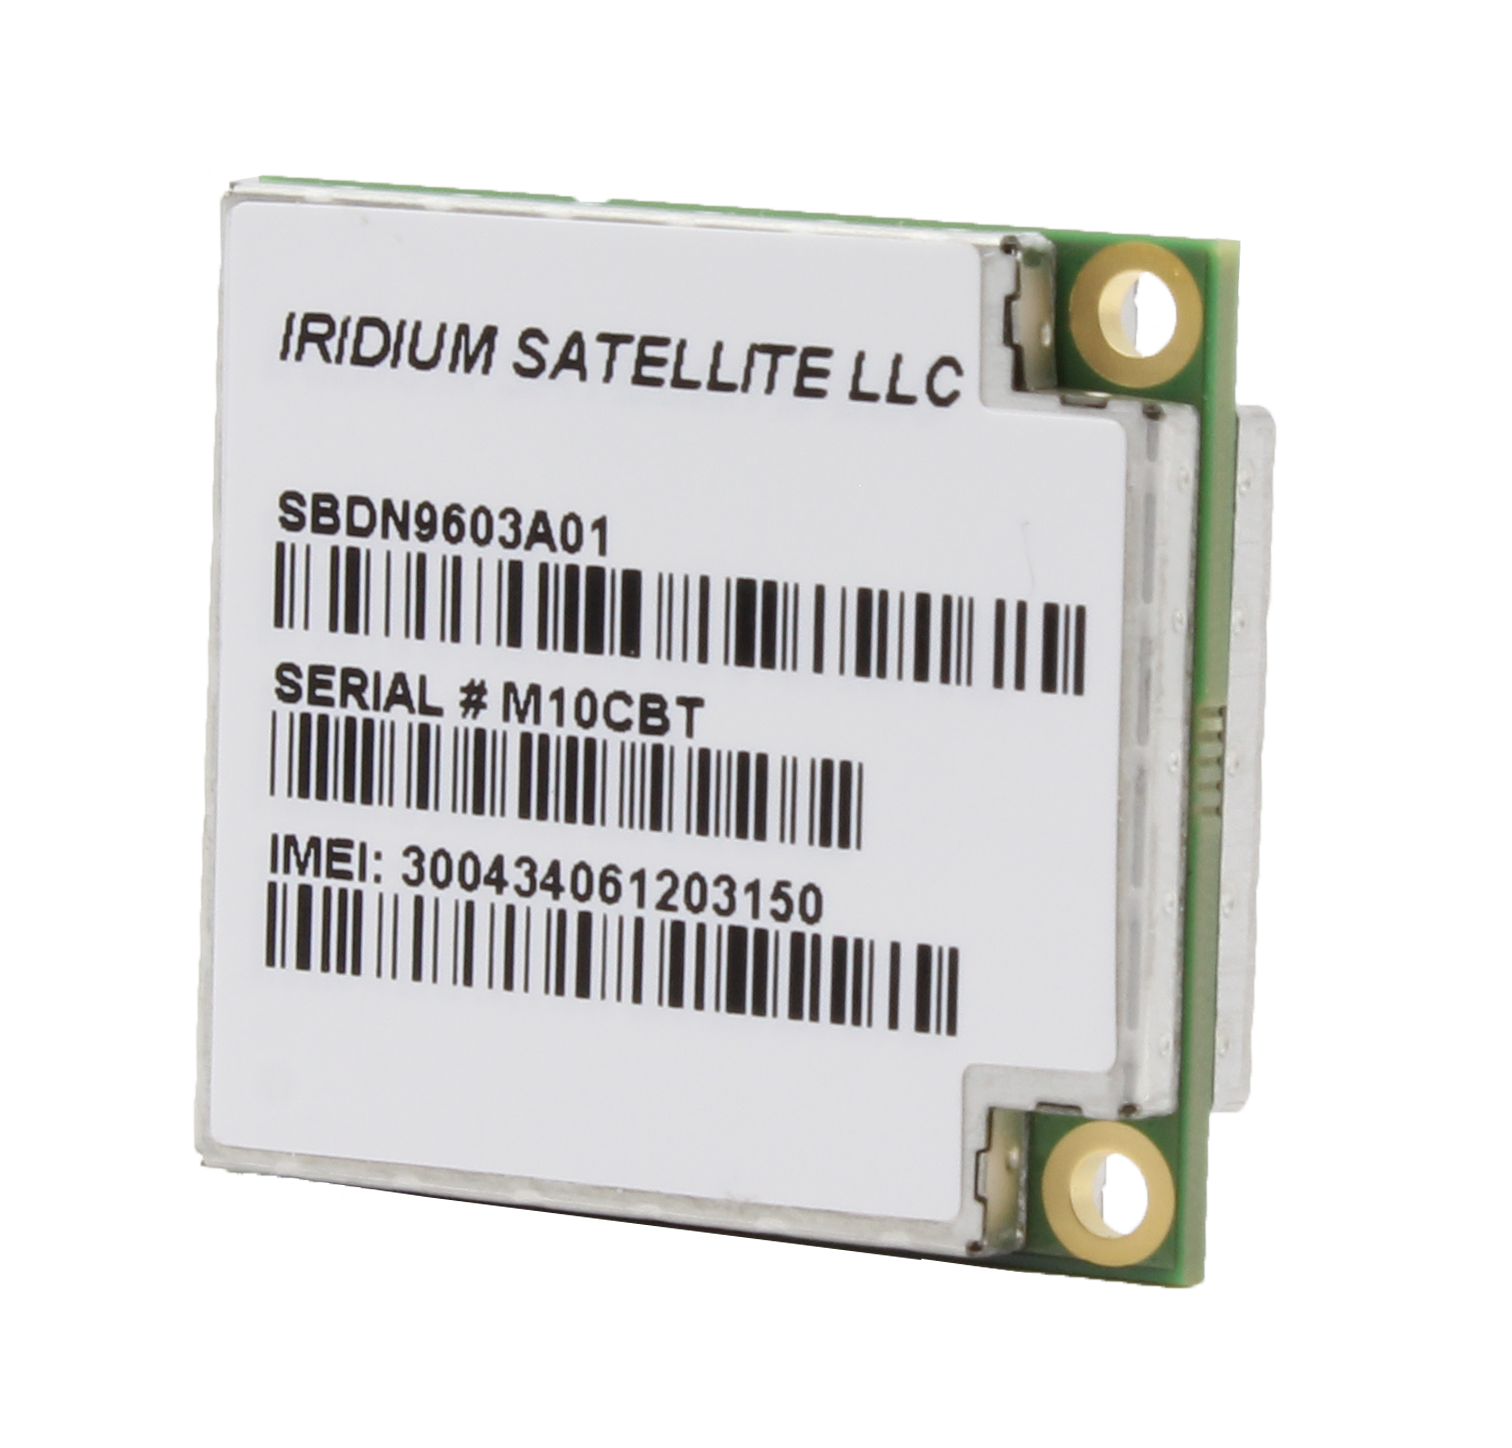
\includegraphics[width = 3cm,height=3cm]{9603.png}};
    \begin{scope}[x={(image.south east)},y={(image.north west)}]
        \draw[color=black, ultra thin,fill=white] (0.0,0.0) rectangle (0.21,0.16) node[pos=.5] {C};
    \end{scope}
    \end{tikzpicture}
    \end{subfigure}%
    \hfill
    \caption{Examples of popular iridium modems selected for remote communications. The 9522B modem (A) (image source: \cite{9522B}), 9602 modem (B) (image source: \cite{9602}) and 9603 modem (C) (image source: \cite{9603})} 
    \label{fig:irid_modem}
\end{figure}
Iridium is a Satellite Network with global coverage and a variety of modems for various IoT uses. The company offers 4 main data services which put constraints on data transmission rates, bandwidth and modem selection. This is shown in table \ref{tab:iridium service}. Furthermore, a full description of these modems are shown in table \ref{tab:ir_devices}. \par 

%figure of open-source buoy using the modem
Unanimously, all devices use the Iridium satellite network for remote communication with the Iridium 9602/3 SBD modem being used the most.  This choice is justified for its small form factor, low power and easy interfacing as shown in table \ref{tab:ir_devices} however it suffers greatly from limited bandwidth having a maximum transmission size of 340 bytes. Systems that use these modems for transmission of wave data rely on complex data processing algorithms and therefore do not transmit the raw time series. The only notable exception to this is the wave buoy developed by\textcite{doble2017robust} which continuously transmitted AHRS and IMU Time Series data once every minute. For this purpose, they used the 9522B modem which allowed for continuous transmission using the RUDICS data service. This modem, along with the SBD modem used for the SWIFT Buoy also has a much larger SBD data buffer (1.92KB) However this comes at the cost of much higher power consumption and significant price increase.  

\subsection{Power Supply}

Table \ref{tab:device_power_source}  shows the power supply strategies of each devices. All systems use batteries as a source of power. Most systems opt for off-the-shelf Alkaline or Lithium-based batteries except for the Buoy by M. \textcite{doble2017robust} which uses a lead-acid battery. Systems deployed in the Arctic Marginal Ice Zone have been designed with a recharging system such as a solar Panel in the case of WII Buoy and Doble Buoy, however, most long-range deployment buoys have opted for non-rechargeable systems composed of Lithium Thionyl Chloride (LISOCL2) or Alkaline batteries. In the case of the high-power buoys (SIMB, WIIOS, NDWB, Polar ISVP) an array of 3.3V -3.7V cells is connected to provide a nominal voltage in series with a regulator to provide a stable output. The strategy for each system is to pack as many batteries in as possible to satisfy the long-term energy requirements.

\subsection{Electronics subsystems}

Component selection for each system is based on the original mission for each buoy. These objectives are shown in  table \ref{tab:device_deployment}. There is significant reporting of devices used in the Antarctic Marginal Ice Zone. However, the more high power devices (i.e. SWIFT, SKIB and NDWB ) have been focused more on the Arctic marginal ice zones. Technology developed for the Antarctic Ocean typically focuses on ice drift and environmental sensing. WIIB was developed using open-source hardware while WIIOS was developed using off-the-shelf components. Both systems aimed to provide a low-cost solution for Wave in ice measurements,  Systems designed specifically for drift will have scaled-down processors, cheaper IMUs with more accurate, more expensive Temperature Sensors and GPS where systems designed specifically for wave measurements have more powerful, sometimes multiple, processors and advanced IMUs with cheaper tracking and Environmental sensing technology. 

The components selection for each system is shown in table \ref{tab:device_components}. The Doble buoy for instance builds its system around the dominant sensor i.e. the AHRS IMU with a single processor controlling all the peripherals as well as allowing for data processing. Drift Loggers such as Trident, and Polar ISVP feature sparser sets of electronics with smaller, lower-powered processors for Power control and peripheral control, In contrast, WIOS and WII Buoy compartmentalise subsystems with a cluster of processors handling different aspects from the buoy. This shows a focus on computation rather than sensing as multiple controllers are used to allowing the main processor to implement advanced Digital Signal processing. SWIFT Buoy appears as the outlier as the system is built around a dedicated data logger i.e. The Sutron Xpert with an integrated processor and Satellite communication link abstracting data processing strategies on the buoy side. The SIMB buoy has the most advanced and largest number of sensors of all the buoys. A commonality amongst the buoys is the use of off the shelf components and processors. A predominant feature, the GPS is an Adafruit MTK339 device that is low cost as well as SAMD Chips, Raspberry Pis and Arduino boards whereas, for Trident and MetOCean, more expensive solutions are used. This shows that developers have opted for ready-made that components that are auxiliary to the main measurements. This should explain why some components on a system are more advanced than others.

\subsection{Polar Performance}

This section outlines the deployment of the systems in the Arctic/Antarctic marginal ice zones and compares the survivability and performance of each system. The focus of this section will be predominantly on devices deployed in the marginal ice zone. Table \ref{tab:device_components} shows the significant deployment locations in the Arctic and Antarctic sea ice zones as well as the deployment objectives of each device.

\subsubsection{Ice Buoy Performance}

\begin{figure}[H]
    \centering
    \begin{subfigure}[b]{0.45\textwidth}
                 \begin{tikzpicture}
             \node[anchor=south west,inner sep=0] (image) at (0,0) {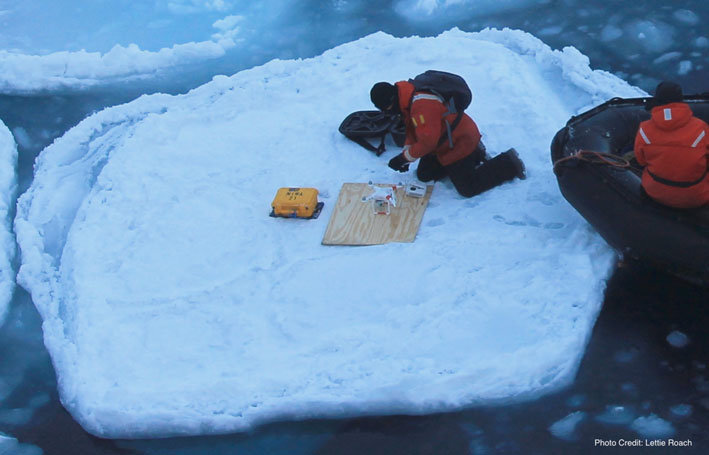
\includegraphics[width = 6cm,height=8cm]{WIIOS.png}};
    \begin{scope}[x={(image.south east)},y={(image.north west)}]
        \draw[color=black, ultra thin,fill=white] (0.0,0.0) rectangle (0.21,0.16) node[pos=.5] {A};
    \end{scope}
    \end{tikzpicture}
    \end{subfigure}%
    \hfill
    \begin{subfigure}[b]{0.45\textwidth}
                      \begin{tikzpicture}
             \node[anchor=south west,inner sep=0] (image) at (0,0) { \includegraphics[width = 6cm,height=8cm]{Basket.jpg}};
    \begin{scope}[x={(image.south east)},y={(image.north west)}]
        \draw[color=black, ultra thin,fill=white] (0.0,0.0) rectangle (0.21,0.16) node[pos=.5] {B};
    \end{scope}
    \end{tikzpicture}    
    \end{subfigure}
    \caption{ Examples of different deployment protocols for ice tethered devices. In regions of consildated ice in favourable conditions, manned crews will step foot on the ice to deploy the device (A) (image source: \cite{kohout2020observation}), in unfavourable conditions, devices may deployed from a basket attached to a crane (B). A manned crew will lower the buoy on a suitable ice floe from the safety of the basket (image source: author) }
    \label{fig:deploy}
\end{figure}
\textcite{kohout2015device} deployed 5 Wave in Ice Observational Systems in the East Antarctic marginal ice zone during the Spring\footnote{1st deployment occured September 2012 \cite{kohout2015device}}. 3 devices were deployed by helicopters on ice floes while 2 devices were deployed via the ships crane. \textcite{kohout2015device}
note that deployment via crane was successful in spite of 7m swell and 25$m.s^{-1}$ winds. The device was fitted inside a pelican box with a sealed membrane surrounded by a tire for protection and flotation in case of melting \cite{kohout2015device}. Consequently, this places the buoy directly on the surface of the floe rendering it susceptible to snow build up and flooding as mentioned in the previous sections.  After deployment, the crew received 600 samples of data over 39 days in total. However, the first device failed 20 hours after deployment coinciding with the first large wave event captured the buoys \cite{kohout2015device}. The second large wave event resulted in the failure of two more systems just 9 days after deployment \cite{kohout2015device}. The 4th buoy lasted for 17.5 days. The final buoy survived the longest at 39 days. As a result only 1 device lasted for the expected time with the majority of data captured during calm events. Two additional WIIOS buoys were deployed by \textcite{alberello2019drift} during the winter \footnote{first deployment occured in July 2017 \cite{alberello2019drift}}. Here, the buoys lasted significantly shorter than the previous deployment. The first system survived for 8 days while the second system survived for 3 weeks in spite of measures taken to place the device in power saving mode \cite{alberello2019drift}. This was achieved by lowering the sample period from to 2 hours. Consequently, the lower temporal resolution resulted in a significantly reduced accuracy of the ice deformation calculations \cite{alberello2019drift}. However, despite this low resolution, by operating at a temporal scale of 3 hours or less \cite{alberello2019drift}, one can effectively and accurately capture ice drift speed as well as the oscillations surrounding the movement. Additionally, \textcite{vichi2019effects} and \cite{albarello2020drift} discuss the deployment of 2 Wave in Ice Observation Systems dissimilar to the ones by \cite{kohout2015device}. 2 devices were deployed on two separate 3m Ice floes 100km from the ice edge \cite{albarello2020drift}. One System survived for 8 days and 18 hours while sampling every 15 minutes before transmission ended \cite{albarello2020drift}. The second buoy however, survived for 6 days sampling every 15 minutes until it switched to power saving mode surviving for a total time frame of 3 weeks. \textcite{vichi2019effects} deployed a second pair of WIIOS buoys in a similar method to \cite{alberello2019drift} however, the first buoy stopped responding after 3 days while the second buoy survived for only 16 days \cite{vichi2019effects}. While the buoys survival is largely attributed to power optimization, the lifespan could be influenced by the selection of the ice floe. Ice floe size and proximity to the ice edge affect the exposure of the floe to open-ocean processes and storms \cite{vichi2019effects}. This could result in failure due to ice mechanic which is discussed in section \ref{ch2:sec3_failiure}. \par 

\textcite{rabault2019open} deployed the Waves in Ice Buoy on land-fast ice to test the device's performance in the Antarctic. In a similar fashion to the WIIOS buoy, the device was placed in a pelican case and attached to a flotation device, however, expected survival time for the device was significantly lower: a maximum of 8 days \cite{rabault2019open} of continuous operation. The buoys by \textcite{kohout2015device} were designed to be expendable\cite{alberello2019drift} whereas the buoys by \textcite{rabault2019open} were designed to be retrievable. Additionally, the WIIB devices were deployed in the summer\footnote{First deployment date: December 2019 \cite{rabault2019open}}. 2 devices were deployed in proximity however an ice break event resulted in the separation of the devices. The devices survived for 2.5 weeks \cite{rabault2019open} which \textcite{rabault2019open} attribute the failure to the devices having been crushed by ice and wave activity. Despite this, the devices were able to record significant wave events and maintain a fully charged battery throughout the deployment which \textcite{rabault2019open} attributes to the solar panel. 

\par \textcite{doble2017robust} alludes to series of environmental considerations when designing the NDWB systems. One such consideration is the frosting over/ rimming of the device due to freezing ocean spray. Additionally, auxiliary power sources (i.e. Solar panels) would need to account for long periods of no cloud cover \cite{doble2017robust}. Since the buoys were deployed by a manned crew, the design also had to account for ease of handling by the crew and not be too heavy \cite{doble2017robust}. The mechanical enclosure consisted of a float and a keel with the electronics contained above the surface in a dome. 20 Buoys were deployed in the Arctic marginal ice zone with each device anchored by drilling a hole in the ice and placing the keel inside. 19 buoys survived the deployment with 1 system failing to boot. The buoys survived for extremely long periods with 12 systems surviving for 200 days off a single alkaline battery pack \cite{doble2017robust}. 7 systems ran for 70 days on alkaline batteries before switching over to solar power. During this period, devices transmitted continuously over the Iridium network and were able to interpolate sea ice phases (see Section \ref{chapter2:subseclcs}) from the tilt of the buoy \cite{doble2017robust}.

\subsubsection{Reasons for Failure}
\label{ch2:sec3_failiure}
\begin{figure}
    \centering
    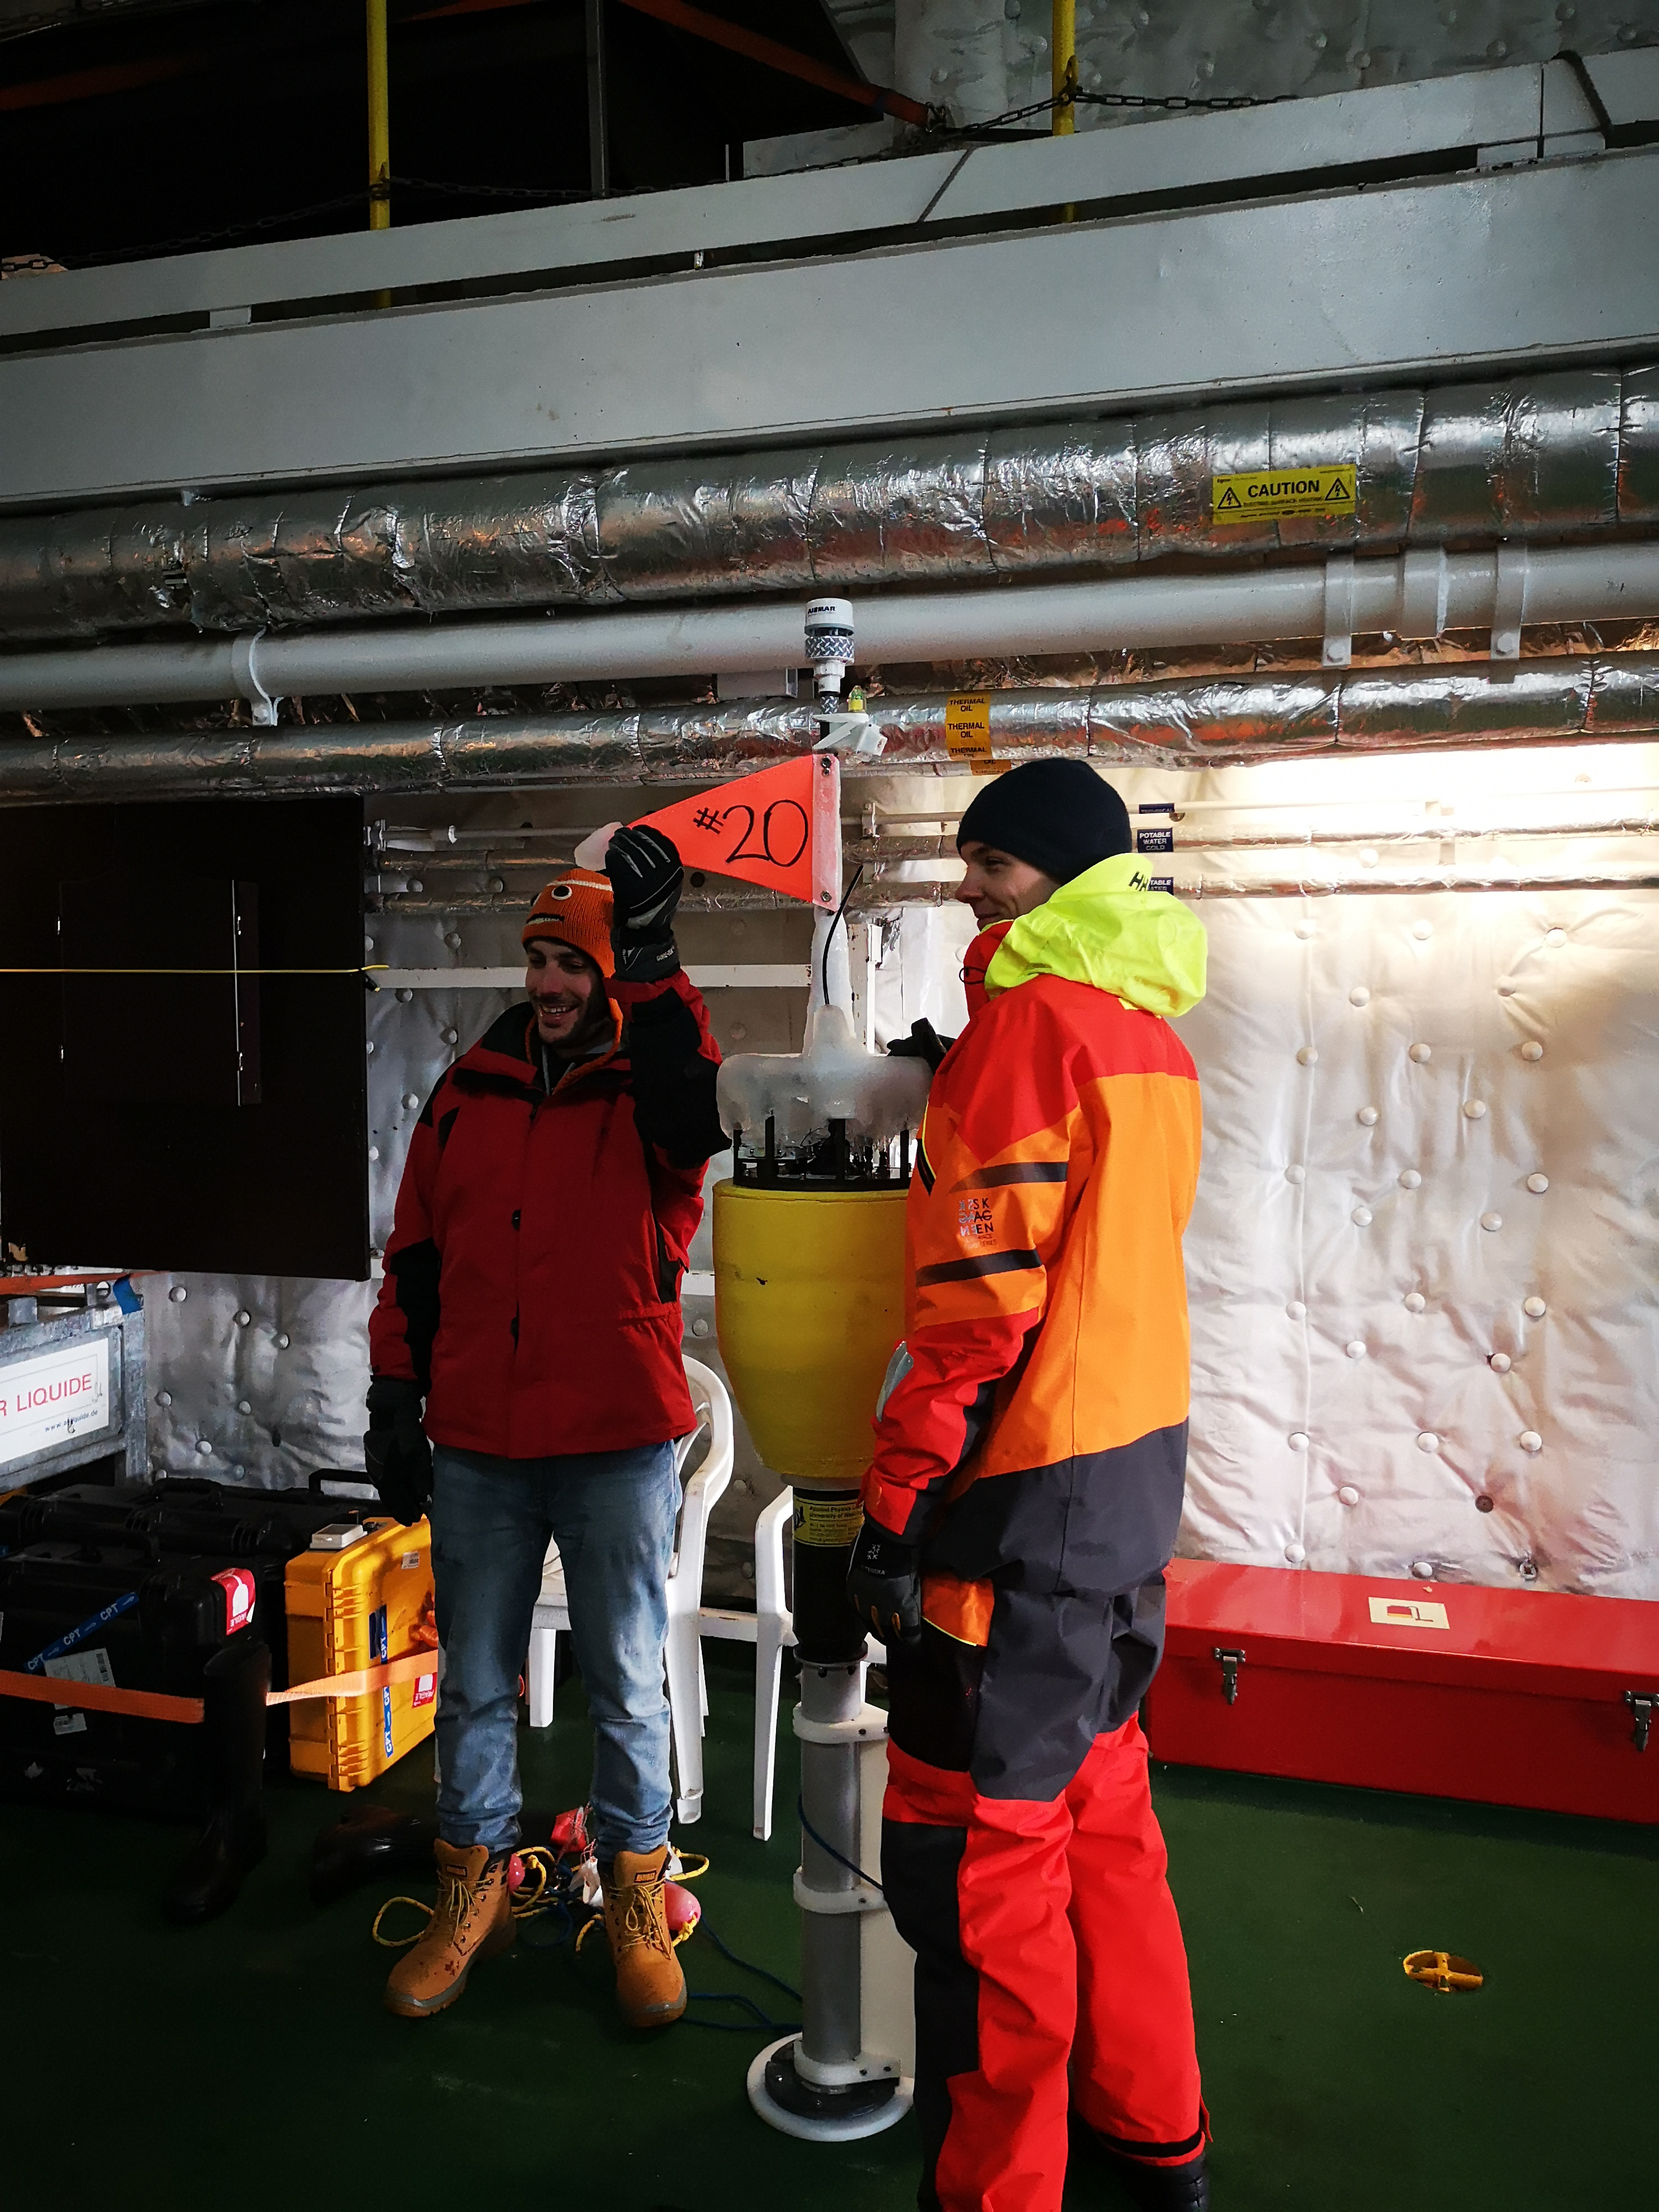
\includegraphics[width = 8cm, height = 6cm]{swift_fail.jpg}
    \caption{During the 2019 SCALE winter expedition, a SWIFT device was retrieved early due to lost communication with the host. This failure was attributed to a build up of ice along the the rim from ocean spray. Photo taken by author.}
    \label{fig:swift_fail}
\end{figure}
Eventually, the systems by \textcite{doble2017robust} lost transmission 300 days after their deployment. This can be attributed to the depletion of the alkaline battery packs. The solar powered lead acid battery voltage eventually dropped below the alkaline battery voltage due to the lack of consistent solar coverage \cite{doble2017robust}. Additionally, sub zero temperatures have a tendency to reduce battery capacities by up to 50\% \cite{doble2017robust} however, \textcite{doble2017robust} found this estimate to be over conservative. Systems by \textcite{kohout2015device} and \textcite{doble2017robust} encountered similar failures with devices eventually depleting the on-board batteries. Additionally, \cite{alberello2019drift} attribute failiure of the first WIIOS system to the battery being depleted.\par 

Additional sources of failure experienced by \textcite{doble2017robust} include ice convergence. The systems were subject to ice-mechanics and as a result, ended up crushed by the floes due to rafting or buried under ice \textcite{doble2017robust}. These failures were identified when more than one system suddenly went offline. Devices also experienced freeze-over or were buried under snow which resulted in the devices going offline for temporary periods \cite{doble2017robust}. Additional evidence of rafting and ridging was captured by webcams on the buoy shortly before transmission ended \cite{doble2017robust}. Buoys that survived the spring melt refroze during the gradual refreezing of the ice. During the second cycle, none of the buoys rebooted when the ice melted in the spring \cite{doble2017robust}. Finally, the buoys developed by \textcite{kohout2015device} and \textcite{rabault2017measurements} sit in close proximity to the ice floes. As discussed previously, during the winter cycles, snow accumulates on the surface that can reach up to 1m in height. This snow formation can result in flooding where the floe becomes submerged. Prolonged burying under snow may have resulted in the device freezing over thereby losing contact while prolonged contact with the seawater may have resulted in the buoys failing on several occasions (\cite{kohout2015device} \cite{vichi2019effects} \cite{albarello2020drift} \cite{rabault2019open})\par 

Finally, \textcite{vichi2019effects} discuss the findings surrounding the failure of the first WIIOS system. \textcite{vichi2019effects} observed a major cyclonic event. The cyclone formed on the 2nd July 2017 and achieved lysis on the 5th July 2017 which coincided with the buoy deployment. Following the event, four more cyclonic events were recorded with three explosive cyclones \cite{vichi2019effects} characterising a change of pressure over 24 hours. During this time, \textcite{vichi2019effects} observed winds speeds of up to $33 m/s^{-1}$ while noting that the air temperatures had increased to values "close to melting" \cite{vichi2019effects}. Additional observations found an increase in significant wave height in the activity. These conditions indicate deformation \cite{vichi2019effects} which may have subjected the buoys to forces experienced by \cite{doble2017robust} during their arctic deployment which were verified against the temperature and pressure readings of the 2nd WIIOS during the cyclonic event. The buoys were deployed close to the ice edge exposed to greater open ocean processes and cyclonic activities than other semi-consolidated and consolidated regions \cite{vichi2019effects}. As a result, air advection, storms and large wave movement delay the consolidation of sea ice considerably \cite{vichi2019effects}. Hence, the ice floes were more likely to experience rafting, ridging \cite{icedefinition1992}, extended flooding, and freezing over which may have caused the failures of the WIIOS buoys.
\newpage
\section{Measurement of External Forces and Effects on Numerical Models}

\subsection{Measurement of Wave data using Accelerometers}

Most of the aforementioned metocean systems focus on measuring sea states and ocean processes. Common measurements of interests are significant wave height and dominant wave frequency \cite{williams2013wave}. Also, Wave data can be analysed in terms of its power spectral density. The two main methods for wave data analysis presented in this section are the Kuik Method and the Welch Earle Method

\subsubsection{Kuik Method}

 The Kuik method, developed by \textcite{kuik1988method} is a computational technique for measuring and determining the directional characteristics of ocean waves. Measurement of these characteristics are derived from the pitch and roll of an ocean buoy are measured. By using an accelerometer, gyroscope or an inertial measurement system to measure the slope and heave of the 3 axes \cite{kuik1988method}, it is possible to reconstruct the sea state given a set of data provided the data is of a specific length sampled above the Nyquist frequency of dominant ocean swells. A major advantage of the Kuik method is that the parameters are estimated directly from the Fourier transform of the measured signal \cite{kuik1988method} without assumptions about the model. Should the algorithm be used to measure waves in ice, no information is required about the dynamics of the model of the ice floe. This greatly improves the accuracy since ice floes can vary in width, distribution and area as well as change shape due to collisions, freezing and melting. Wind waves are described using a two-dimensional energy spectrum $E$ with wave energy spread over a frequency $f$. The normalised distribution of energy over direction is defined according to \textcite{kuik1988method} as
 \begin{equation}
     D_f(\theta) = \frac{E(f,\theta)}{\int_0^{2
     \pi}E(f,\theta)d\theta}
 \end{equation} 
 
 Finally, by computing the model per frequency, the distribution simplifies to $D(\theta)$ which can be approximated by a Fourier series with 4 terms \cite{kuik1988method} derived from the pitch, roll and heave of a buoy. Finally, the model can fully characterise the wave spectrum by calculating the following parameters from the Fourier coefficients:
 
 \begin{enumerate}
    \item mean wave direction $\theta_0$
     \item directional width $\sigma$
     \item skewness $\gamma$
     \item kurtosis $\delta$ 
 \end{enumerate}

The accuracy of the mean wave direction and width is affected by noise in the sampled data. small RMS values of noise can result in rapid increases of directional width by 1\% to 5\% \cite{kuik1988method}. Additionally, pitch and roll buoys are not free particles. They have an associated mass and therefore an associated inertia \cite{kuik1988method}. This results in a phase shift of the Fourier term by $\phi_i i \in {x,y,z}$  in the first harmonic \cite{kuik1988method}. This shift can result in an error of $0.5^\circ $ for $\sigma > 25 ^\circ $ to $1^\circ \text{ for } \sigma < 10^\circ $ \cite{kuik1988method}   

\subsubsection{Welch-Earle Method}

The Welch-Earle Method is an algorithm for calculating either directional and non-directional wave data depending on the assumptions of the input data \cite{earle1996nondirectional}. Data is derived from the vertical acceleration, roll and pitch of a buoy oriented perpendicular to the surface on either a vertically stabilised platform or a hull-fixed platform \cite{earle1996nondirectional}. Directional wave data is determined from both the acceleration, roll, pitch and heave from the buoy while non-directional wave data is calculated from time-series acceleration only. In this method, a digital time series representation of the vertical Acceleration along with 2 orthogonal Gyroscope measurements and Magnetometer readings relative to the earth’s magnetic field is obtained. The method accounts for the response function of the buoy and provides corrections to phase differences as a result of the buoy's inertia \cite{earle1996nondirectional}. Full directional and non-directional wave data is characterised by calculating the spectra and co-spectra of the time series data. The first part of the method is developed by \textcite{welch1967use} and is used to calculate the power spectral density.
Given a discrete time series data X(j) with a power spectral density P(f), |f|< $\frac{1}{2}$.this data segmented into a set of k-bins $X_k(j) | j \in {0,L-1}$ \cite{welch1967use}. Each bin is multiplied by a selected window function W(k) of length L. Additionally, Bins are taken with a 50\% overlap to produce better statistical averages \cite{earle1996nondirectional} The Fast Fourier Transform (FFT) of the result is taken to for a periodograms $I_k$ \cite{earle1996nondirectional}. Finally, the new power spectral estimator $\hat{P}(f_n)$ is calculated by taking the average of the K periodograms as shown in \textcite{welch1967use}

\begin{equation}
    \hat{P}(f_n) = \frac{1}{K}\sum^K_{k=1}I_k(f_n)
\end{equation}

where 
\begin{equation}
    f_n = \frac{n}{L} | n \in 0,1,2... \frac{L}{2}
\end{equation}

Detrending is used to account for the effects of buoy motion on the time series. The inertia of the platform results in non-zero mean trends often as a result of constant wind or currents acting on the hull of the buoy \cite{earle1996nondirectional}. These must be discarded before the spectrum and co spectra are calculated. The resolution of the accelerometer is important for accurately tracking acceleration \cite{kohout2015device}. If the resolution is too small, low accelerations will not be recorded resulting in incorrect vertical accelerations being calculated. \textcite{kohout2015device} found that a low-resolution IMU was unable to reliably flag that it had exceeded a boundary condition and hence it was discarded \cite{kohout2015device}\par 

The spectra and co-spectra of the directional and non-directional wave series can be calculated by computing the spectrum $S(x)$ as a function of frequency and direction (as is similar to the Kuik method). \textcite{earle1996nondirectional} show that characterisation of the co-spectra $C(x)$ and spectrum$S(x)$ can be achieved by calculating the first 4 Fourier coefficients. Finally, the sea state can be represented by calculating the following parameters

\begin{enumerate}
 \item Longuet-Higgins directional parameters
    \begin{enumerate}
        \item $a_0$
        \item $a_1$
        \item $b_0$
        \item $b_1$
    \end{enumerate}
    \item Significant Wave Height $H_0$
     \item Dominant Wave Period $T_p$
     \item Total Degrees of Freedom $TDF$
     \item Average zero-crossing period $T_{av}$
     \item Zero-crossing period $T_{zero}$
\end{enumerate}
 This approach brings into account the possibility of spectral leakage however, this can be greatly minimised by sampling above the Nyquist frequency of the upper Wave frequency band (generally taken to be 0.5Hz) for a minimum of 1000 seconds (about 16 – 17 minutes). Additionally, spectral leakage can be reduced by selecting a window function with a gradual taper such as a half cosine or Hanning taper \cite{welch1967use}\par

\subsubsection{Implementation}
As mentioned previously, systems such as WIIOS and WIIB have built their purpose around wave measurements and therefore have specified High Powered, High Accuracy IMUs for wave measurements. However, WIIOS buoy separates itself from WII Buoy by having a cheaper complimentary 9 d0f IMU to complement the measurements. SWIFT Buoy and the DOBLE buoy use an integrated system known as an Inertial Navigation System. This device contains a GPS and an Onboard processor for RTK fusion and Kalman filtering whereas other devices use an external processor for filtering. The SIMB Buoy is the only buoy on the list that has an IMU for non-wave related measurements. It uses a cheaper Bosch BNO055 which is used solely for measuring the orientation of the device.

\subsubsection{Software processing}

\par{WIIB}	

Raw Time series is passed through an Extended Kalman Filter running at 800Hz than a low pass filter. Wave Spectral data is calculated using the method by \textcite{earle1996nondirectional} where Co-Spectra is calculated using the Method by \textcite{kuik1988method}. Significant wave height is calculated through double integration. A Fast Fourier transform is applied to the data series to achieve this.
\par{WIIOS}

Data is filtered using a Butterworth filter with a cut-off frequency of 2Hz. Significant wave height is calculated by double integration using a Fast Fourier Transform. Spectra is calculated using the method by \textcite{earle1996nondirectional}.

\par{NDWB}

The double buoy is unique as it does not directly calculate wave parameters. However, the raw time series is filtered using an Extended Kalman Filter running at 10Hz

\par{SKIB}

Data collected from a sample window is processed using a classical RC filter to attenuate frequencies below 0.04Hz. \textcite{earle1996nondirectional} Spectra and Co-Spectra  Calculation is then applied.

\par{SWIFT}

The Swift buoy is the only device that uses multiple sensors for sea state calculation. First, data is collected more frequently in short intervals (9 minute sample periods every 12 minutes) which include Doppler Profiles, Camera images and IMU data. The INS System outputs a Real-time kinematic (RTK) fusion data series where IMU data is passed through a Coning \& Sculling Extended Kalman Filter running at 1KHz while the Doppler profiler is sampled at 8Hz. Turbulence profile is calculated through time-averaged data fitting of the Doppler profiler. The current state is calculated using the Stokes drift Equation over time-averaged velocity series. Finally, Wave information is calculated from an image of the sea state.

\par{SIMB}
No Clear Data processing strategy is available in the literature. This may be due to the non-critical nature of the IMU.

\subsection{Measurement of Ice drift using GPS}

The approach towards studying ice drift is typically performed using the techniques presented by \textcite{hibler1979dynamic} \footnote{See Numerical Modeling} where kinematic data is used to study ice drift dynamics and calibrate the ice drift model.\textcite{lepparanta2001sea} present two methods for data. The first method utilises measurement beacons are attached to the ice floes and used to track trajectories. The second method uses imaging devices such as radar, and satellites to determine ice displacement \cite{lepparanta2001sea}.\par

Each ice floe follows a unique trajectory \cite{lepparanta2001sea}  and individual trajectories combine to form a continuum. It has previously been believed that Sea Ice drift has been linked strongly to significant wave events \cite{alberello2019drift}. An experiment was conducted by \textcite{alberello2019drift} to measure the drift of sea ice during a cyclone event. Here it was found that wind velocity is the dominant driver of sea ice drift \cite{alberello2019drift} causing ice drifts of up to $0.75 m\cdot s^{-1}$ \cite{alberello2019drift}. Sea Ice drift speed is extremely sensitive to sampling rates. \cite{alberello2019drift} where sampling rates of 6 hours can underestimate the ice velocity by 5\% \cite{alberello2019drift} and up to 20\% for 12-hour sample rates. The consequence is reduced, near unusable, estimates of sea ice velocity components as well as drag coefficient and wind factor estimates. High temporal resolutions are capable of capturing important, inter-daily such as Ice oscillations. \textcite{alberello2019drift} state that to accurately capture Sea Ice behaviour, a temporal resolution of at least 3 hours is required \cite{alberello2019drift}. This not only allows for the capture of accurate drift speeds but provides an accurate characterization of Instantaneous velocities and Coriolis forces \cite{alberello2019drift}. Satellite observations OSI-SAF and METSAT are unsuitable for measurements hence a need arises for in -situ drift measurement devices. The GPS technology has been the standard for ice drift measurement. Current measurement sensing platforms such as those developed by \textcite{kohout2015device}, \textcite{rabault2019open}, \textcite{doble2017robust} and proprietary sensing technologies; Trident Buoy, SWIFT Buoy, Metocean. The GPS is set to measure data at relatively high temporal resolutions ranging from 15 minutes \cite{alberello2019drift} to 25 minutes \cite{rabault2019open}.

\subsubsection{Overview of GPS}

The principles that govern GPS have remained unchanged since its inception in 1973 \cite{spilker1996global}. The system consists of a satellite constellation that constantly broadcast their estimated position. A GPS device determines its position by matching a user-generated signal to that of 4 received satellites and comparing the phase difference to an on-board crystal oscillator \cite{spilker1996global}. This technique is called ranging and 4 satellites spread in a uniform geometry will allow for a device to calculate latitude, longitude, altitude and time to a relative degree of accuracy. The number of unknown signals correlates to the number of satellites required. Generally, a GPS device will have a lesser degree of accuracy than the satellites hence, an incoming signal can be used to correct the device's clock \footnote{provided altitude or time are already known \cite{spilker1996global}}.To accurately predict the satellite's trajectory, Satelite ranging is performed by a network of global monitoring which calculate the future position and send it back to the satellite. GPS signals are transmitted on two frequencies: 1575.42MHz and 1227.46MHz\cite{spilker1996global}. These are synchronously generated signals and allow a device to correct for ionospheric distortion. These bands carry modulated signals which are as follows: \cite{spilker1996global}


\begin{enumerate}
    \item Clear Acquisition Code:  This is a short code transmitted at 1.023 MHz and is used to request the Standard Positioning Service or SPS.
    \item Precise (P) Code: this is a much longer acquisition code. This signal is transmitted at 10.23MHz which is 10 x the rate of a CA code. This results in a much more accurate signal with less noise. This signal allows for the acquisition of Precise Positioning Service. However, this service is not available to unauthorized users and cannot be spoofed. As a result, this signal requires additional decryption.    
\end{enumerate}

\textcite{spilker1996global} also mention that military operators can degrade GPS signals which result in decreased accuracy from 20m up to 100m. The reduction of these accuracies requires differential GPS techniques, however, for the sake of this project. \par
once the acquisition signal is transmitted, the GPS device begins modulating at 50 bit/s. This allows the satellite to transmit its position as well as clock correction information to the device.\par
The GPS satellite constellation consists of 24 GPS satellites. These are configured into 3 rings of 8 satellites orbiting at different latitudes. The orbital altitudes were selected as 10.98 Nautical Miles \cite{spilker1996global}. This altitude was chosen to optimize user visibility with the number of crossings over United Sates ground stations, and cost of launching the satellites \cite{spilker1996global}. These satellites carry onboard atomic clocks for stability at $1\times10^{13}$ resolution. This allows for extremely accurate signalling as well as allowing for much more predictable time and position signals \cite{spilker1996global}. To achieve this, these atomic clocks are made out of either Cesium or Rubidium. Also, a frequency correction at $4.5\times10^{10}$ is provided to correct for relative shifts. \par
\subsubsection{GPS Error Modeling}
As mentioned before, the accuracy of the GPS signal is greatly affected by earth effects and satellite distribution. The main source of distortion is attributed to the earth's Ionosphere \cite{spilker1996global}. The ionospheric free electronics cause a delay in the modulated signal which is proportional to the sum of electrons along the signal's trajectory and inversely proportional to the signal's frequency squared. This delay is modelled as the product of a theoretical $90^\circ$ delay (Zenith delay) and a function of the elevation angle (obliquity factor). This results in a ratio of between 1.0 to 3.0 at small elevation angles \cite{spilker1996global}. This results in delays of 3m (often at night) to 20m (after midday). These delays are usually resolved by Satelite correlated positions. Correction can be performed in one of two ways:
\begin{enumerate}
    \item Transmission of Ionospheric model parameters as part of the message to the device and calculating the offset using that
    \item Using the two previously mentioned transmission frequencies directly measuring the delays in each broadcast frequency and estimating the position using the equation:\cite{spilker1996global}
    \begin{equation}
        1.546(delay_{L1} - delay_{L2})
    \end{equation}
\end{enumerate}

Navigation errors are characteristic of GPS performances. These errors are affected significantly by Satelite spread and ranging errors. Assuming the incoming signal is uncorrelated with a mean of zero, the RMS positional error is calculated as:
\begin{equation}
    RMS_{error} = (\text{Geometric Dilution})(\text{RMS Ranging errors})
\end{equation}

The geometric Dilution is modelled by estimating the precisional dilution of the spatial and temporal dimension measurements. This value estimates the quality of the GPS signal and is inversely proportional to the volume of the shape formed by 4 satellite \cite{jwo2001efficient}. Jwo (2001) outlines the procedure for the calculation of this value. Given a user's position on the earth, the distance from the user to the satellite is characterised by the equation:
\begin{equation}
    r =  s - u
\end{equation}
where $r$ is the distance from the user to the satellite, $s$ is the distance from the earth's centre to the satellite and u is the distance from the earth to the user. By measuring the propagation time from the user to the satellite, The absolute distance $||r||$ can be calculated and hence, the pseudo-range can be calculated as
\begin{equation}
    \rho_i = ||s_i-u||+ct_b + v_{\rho_i}
\end{equation}
where $\rho_i$ is the pseudorange for satelite i, c is the speed of light, $t_b$ is  the clock offset and $v_{\rho_i}$ is the noise of the pseudorange measurement and:
\begin{equation}
    ||s_i-u|| = \sqrt{(x_i - x_u)^2+(y_i-y_u)^2+(z_i-z_u)^2} \text{ for } i \in 1,2,3...N \label{los}
\end{equation}
where N is the number of satelites and $(x_i,y_i,z_i)$ is the 3 dimensional position of satelite i. This represents a non-linear relationship for the line of sight of a satelite.  Jwo (2001) Explains that by creating a Taylor series centered on a nominal user position $(\hat{x_n},\hat{y_n},\hat{z_n})$ and ignoring the higher terms \cite{jwo2001efficient}. It then follows that:
\begin{equation}
    \Delta\rho_i = \rho_i - \hat{\rho_i} = e_{i1}\Delta x_u + e_{i2}\Delta x_u +  e_{i3}\Delta z_u
\end{equation}

The terms $e_{ij}$ represent the line of sight vector $E_i$ whereas the term $\hat{\rho_i}$ is the pseudo-range at the nominal user's position. It follows that the vector $E_i$ can be calculated as follows \cite{jwo2001efficient}.
\begin{subequations}
                \begin{align}
                    e_{i1} = \frac{\hat{x_n} - x_i}{\hat{r_i}}\\
                    e_{i2} = \frac{\hat{y_n} - y_i}{\hat{r_i}}\\
                    e_{i3} = \frac{\hat{z_n} - z_i}{\hat{r_i}}\\
                    \hat{r_i} = \sqrt{(\hat{x_n} - x_i)^2+(\hat{y_n} -y_i)^2+(\hat{z_n} -z_i)^2}
                \end{align}
\end{subequations}

Given n number of satellites, the equation \eqref{los} can be written as a matrix with the following form:
\begin{equation}
   \textbf{z} = \textbf{Hx}+ \textbf{v}
\end{equation}
\begin{equation}
    \Delta \rho _i = \begin{bmatrix}
                        \Delta \rho_1 &  \Delta \rho_2 &  \Delta \rho_3 & ... & \Delta \rho_n
                     \end{bmatrix} 
\end{equation}
where 
\begin{subequations}
                \begin{align}
                    \textbf{H} = \begin{bmatrix}
                                   e_{11} & e_{12} & e_{13}& 1 \\
                                   e_{21} & e_{22} & e_{23}& 1 
                                   \\
                                   e_{31} & e_{32} & e_{33}& 1
                                   \\
                                   ... & ... & ... &  1 
                                   \\
                                   e_{n1} & e_{n2} & e_{n3} & 1
                                 \end{bmatrix}\\
                    \textbf{x} = \begin{bmatrix}
                                    \Delta x_u \\ \Delta y_u \\\Delta z_u \\ c\Delta t_b
                                 \end{bmatrix}\\
                    \textbf{v} = \begin{bmatrix}
                                v_{\rho_1}\\
                                v_{\rho_2}\\
                                v_{\rho_3}\\
                                ...\\
                                v_{\rho_n}
                             \end{bmatrix}
                 \end{align}
\end{subequations}

The Matrix \textbf{H} is $n\times4$ where $n \geq 4$ to calculate all the paramters for GDOP \cite{jwo2001efficient}. We can then solve for the vector \textbf{x} by taking the psuedo inverse of H i.e $\hat{\textbf{x}} = (\textbf{H}^T\textbf{H})^{-1}\textbf{H}^t\textbf{z}$. Hence, given that the psuedo range is linearised, the quality of navigation is taken as the difference between the estimated position and the actual position \cite{jwo2001efficient}.
\begin{equation}
    \Tilde{\textbf{x}} = \hat{\textbf{x}} - x = (\textbf{H}^T\textbf{H})^{-1}\textbf{H}^Tv
\end{equation}
 $E\{\Tilde{\textbf{x}}\Tilde{\textbf{x}}^T\}$ describes the covariance between the errors in the components of the estimated position \cite{jwo2001efficient} and is calculated as 
 \begin{equation}
   E\{\Tilde{\textbf{x}}\Tilde{\textbf{x}}^T\} = (\textbf{H}^T\textbf{H})^{-1}\textbf{H}^TE\{\textbf{vv}^T\} (\textbf{H}^T\textbf{H})^{-1}\textbf{H}
 \end{equation}
 where $E\{\textbf{vv}^T\} = \sigma^2 I$. If all components of $\sigma$ are uncorrelated then the covariance becomes 
 \begin{equation}
     E\{\Tilde{\textbf{x}}\Tilde{\textbf{x}}^T\} = \sigma^2(\textbf{H}^T\textbf{H})^{-1}
 \end{equation}
and thus the GDOP factor can be calculated from the RMS values of $\sigma^2$ i.e.
\begin{equation}
    GDOP = \frac{\sqrt{\sigma_{xx}^2+\sigma_{yy}^2+ \sigma_{zz}^2+\sigma_{tt}^2}}{\sigma}
\end{equation} where $\sigma_{xx}^2$,$\sigma_{yy}^2$,$\sigma_{zz}^2$,$\sigma_{tt}^2$ are the RMS values of the x,y,z time components respectively. THe value GDOP can also be decomposed into the components PDOP,TDOP,HDOP,VDOP which represent the dilution of precision of Position, Time, Horizontal position and vertical position respectively.\par

Ranging errors are shown to come from 6 sources \cite{spilker1996global}:
\begin{enumerate}
    \item Satelite Ephemeris
    \item Satelite Clock
    \item Ionospheric group delay
    \item Trophospheric group delay
    \item Multipath scattering
    \item Hardware/software errors
\end{enumerate}




\subsection{Temperature Sensing and Measurement}

Environmental Sensing plays a pivotal role in predicting earth systemic processes. Tracking major events such as cyclones \cite{vichi2019effects} requires constant monitoring of antarctic environmental conditions. Temperature sensors can help predict atmospheric events such as storms, cyclones and seasonal changes as well as sea ice events such as sea ice melting \cite{kohout2015device} \cite{doble2017robust}. \textcite{doble2017robust} have discussed the significance of sea ice melting. This was considered a significant phase of sea ice and was classified as a phase in the development of their buoy. \par 

Temperature sensing technology is widely used for a variety of applications including food storage, mechanical failure warning systems, transport systems etc. \cite{awtrey2002environmental}. The majority of temperature sensing technology is used for thermal compensation as measurements such as pressure and humidity are dependant on environmental temperature \cite{mansoor2015silicon}. Thermal sensing technology exists in a variety of forms however, choice of sensor is heavily dependant on the application i.e. the object to be measured, the material state and the type of contact with the sensor \cite{mansoor2015silicon}\cite{childs2000review}. There are 3 main categories of measurement techniques \cite{childs2000review}:
\begin{enumerate}
    \item Invasive Measurements: Direct contact with an object of interest. This method is suitable for the measurement of objects in liquid or gas states. This category encompasses thermoelectric devices, liquid in glass thermometers, electronically resistive devices as well as semiconductor devices \cite{mansoor2015silicon}
    \item Semi-Invasive: Using the thermal measurement medium on an object and observing the effects of temperature such as thermal paints. Note: measurements are not directly taken from the object but rather the properties of the medium
    \item Non-Invasive: Object is measured from a distance using a device such as an infrared camera or acoustic thermography
\end{enumerate}
Also, the sensor selection must be based on the range, accuracy, resolution and precision of the device to ensure correct use An overview of different electric sensors is given below \cite{childs2000review}
\subsubsection{Thermocouples}

These devices use the principle of the Seebeck effect. Two conductors are joined at a junction which causes small electrons to flow \cite{pollock2017thermocouples}. This generates an EMF which is proportional to the temperature difference across their junctions \cite{pollock2017thermocouples}. Measurements are made using pairs of these conductors (referred to as thermo-elements \cite{pollock2017thermocouples}) one of the junctions is set to a known reference temperature (usually $0^\circ C$) while the other junction is measured. The resulting voltage is measured as a function of the temperature across the junction. In a practical sense, it may not be desirable to hold the reference voltage at $0^\circ C$, in this case, any reference voltage can be used provided it is fixed, repeatable and known \cite{pollock2017thermocouples}. a non-zero reference voltage will result in a relative voltage change. Hence this must be compensated in the measurement algorithm \cite{pollock2017thermocouples}. These devices have a wide temperature range from (-200 $^\circ C$ to 2000$^\circ C$ \cite{tong2001improving}). Despite this, there are some disadvantages. The temperature-voltage relationship is non-linear \cite{pollock2017thermocouples} \cite{tong2001improving} which can result in more intensive computational requirements as well as inaccuracies. Also, relative temperatures do not result in a stable voltage which gives uncertainty up to 2 $^\circ C$. Despite this, thermocouples are relatively cheap with a fast thermal response. However, this comes with a trade-off of increased noise. Finally, the temperature range of the thermocouple is limited by the metal used. Fortunately, thermocouples come in standard types \cite{tong2001improving} which have an associated range \cite{tong2001improving}
The relationship governing the emf and relative temperature change is shown to be. 
\begin{equation}
    E_{ab} = E_0 + a \Delta T+ b\Delta T^2
\end{equation}

$E_{ab}$ is the emf across the junction formed by conductors a and b. T is the measured temperature. $E_0$ is the reference temperature (a constant),  a and b are constants otherwise known as the relative Seebeck coefficients. These values can be determined by solving the above quadratic and are derived by Pollock (2017) as.
 \begin{subequations}
                 \begin{align}
                     a = \alpha - \beta\\
                     b = \frac{m_A-m_B}{2}
                 \end{align}
 \end{subequations}
 $\alpha \text{ and } \beta$ are constants derived from the open circuit potential of conductors a and b respectively. $m_a\text{ and } m_b$ are the gradients of conductor and b respectively. \cite{pollock2017thermocouples}. 
 \subsubsection{Resistive Temperature Detector}
 
 Resistive Temperature Detectors (or RTDs) consist of metal with a known Temperature Coefficient. The device has a resistance that changes proportionally to the change in ambient temperature \cite{tong2001improving}. These devices are considered the most stable and accurate sensors \cite{tong2001improving} having an uncertainty range of $0.03^\circ C$ to $0.3^\circ C$ depending on the type. However, these sensors are considered more fragile and are largely expensive to obtain. These sensors come in the form of either a wound wire or a metal film with a known resistance at a specific temperature \cite{tong2001improving}. The advantage of these devices is a linear relationship between resistance and temperature. Hence a simple ohmic measurement \cite{tong2001improving} will allow for simple temperature prediction, however, these devices have a low sensitivity which can cause errors of up to $5 ^\circ C$ in this configuration \cite{tong2001improving}. A solution to this is to use four RTDs in a four-wire configuration where 2 wires provide excitement current and two wires connect to a voltmeter. This, however, adds to the complexity of the measurement and requires a more demanding processor. The measurements noise is proportional to the excitation current which causes the sensor to self-heat, According to Tong (2001) must be kept below 1mA to avoid significant noise distortion. Calibration of the sensor is performed against a compensation curve often provided with the device in question.
 \subsubsection{Thermistors}
 
 Modern Thermistors have progressed significantly in the past decade. Up until recently, they have been considered inaccurate with uncertainty ranges of up to 5\% \cite{tong2001improving}. Modern thermistors are capable of providing accuracies of up to 0.01$^\circ$. They consist of a semiconductor that changes its resistance in response to temperature \cite{childs2000review}. They have a faster response time than RTDs and work on the same principle for temperature measurement. However, where RTDs have a Positive temperature coefficient, Thermistors have a negative temperature coefficient \cite{tong2001improving}. These devices can operate over a substantial, albeit relatively limited, range of $-100^\circ - 300^\circ C$. The major trade-off with these devices is the lack of standards \cite{tong2001improving}. Operating the device involves a large degree of uncertainty. Also, these devices are not powerful enough to accurately reach the desired ranges alone. They need to be coupled with similar devices. Finally, the response curve is non-linear. The  relationship between resistance and temperature is \cite{childs2000review}:
 \begin{equation}
     R_T = R_0e^{1 - B(\frac{1}{T}- \frac{1}{T_0})}
 \end{equation}
where $R_T$ is the temperature measured, $R_0$ is the resistance at a known temperature $T_0$, T is the temperature and B is a coefficient based on the properties of the thermistor. Finally, these devices are more prone to noise from excitation current.
 \subsubsection{Silicon Temperature Devices}
 
 Semiconductor temperature devices are suited to applications where the temperature ranges from -55 to 150 $^\circ C$ these devices are capable of providing a stable output with a typical accuracy of $0.8 ^\circ C$. These devices typically consist of diodes and transistors with a bandgap voltage that changes with a change in temperature \cite{childs2000review}. These devices are advantageous in electronic application due to their small form, high accuracy and stability. These devices are relatively simple and have a good sensitivity to changes \cite{childs2000review}. Diodes are typically used in semiconductor devices. Here, the forward voltage drop across the p-n junction is linearly proportional to the Ambient temperature over a certain temperature range (typically 25K - 400k) \cite{childs2000review}. These devices are made out of either silicon or Galium-Arsenide. Silicon is preferred as it has better stability at low temperatures and is cheaper however, this comes at the trade-off of a lower voltage output \cite{childs2000review}. \par These Types of devices are readily available in IC forms and are manufactured in a variety of packages, types and compositions for any application. Typical devices are DS18B20, LM355 or BMP2080. Recent innovations in Silicon sensing have seen the rise of CMOS devices and Micro Electrical-MEchanical Systems (MEMs) being used more frequently \cite{mansoor2015silicon}. While these devices can suffer from deterioration due to self-heating, \textcite{mansoor2015silicon} discuss that the low-power operation of these devices can offset this issue. This is advantageous for systems that are constrained by power consumption. However, a major disadvantage with these devices is that these devices work ideally with a purely DC signal.An AC coupled signal can cause significant errors in the output \cite{childs2000review} \cite{mansoor2015silicon}. These errors can be the result of improper shielding and poor grounding. Hence proper shielding and grounding are required to reduce these errors. Finally, these devices require careful calibration before use.
 
\subsection{Atmospheric Pressure Sensing and Sensors}
Atmospheric pressure is a key measurement for environmental sensing. There has been an increased demand for in-situ environmental monitoring as mentioned by \cite{vichi2019effects} \cite{kennicutt2014polar} \cite{kennicutt2016delivering} \cite{kennicutt2019sustained} \cite{alberello2019drift}. It can provide insight into wind currents and storm events as well as predict trajectories of these storms. Also, pressure characterises the relationship between Atmospheric and ocean air process. The pressure is a Temperature dependant measurement \cite{mansoor2015silicon} and, often, Autonomous platforms couple pressure sensors with temperature sensors on the same Integrated Circuit (IC). One example is the BMP280 environmental sensor developed by Bosch \footnote{More details provided by Bosch Sensortech }. The current state of Pressure Sensing technology is driven towards Miniature MEMs version of large scale devices \cite{eaton1997micromachined}. Most large scale pressure sensors consist of a diaphragm mounted on a device in a known way. The diaphragm is coupled to a device that converts the pressure to a mechanical movement which is then measured using a gauge. These senses often had a secondary sensor that would convert the mechanical movement to an electrical signal which was then measured \cite{eaton1997micromachined}. Other sensors include barometers, bourdon tubes and vacuum pressure gauges. Most MEMs are based on these principles.\par 
\textcite{eaton1997micromachined} discuss the importance of micro-machined pressure sensors and provide an overview of various sensors. These can be classified as piezoresistive, capacitive, optical and resonant each with their pressure relationship.
\subsubsection{Diaphragm Based Sensors}
Previously mentioned, Diaphragm sensors determine pressure by measuring the deflection of a miniature diaphragm. This deflection is converted to an electrical signal. Typically, a reference pressure is provided as a measurement of a sealed chamber or absolute pressure port. Assuming the simplest version of this sensor i.e. a plate of uniform thickness \cite{eaton1997micromachined} The deflection $w$ of the diaphragm is related to the pressure  $P$ by the following equation: \cite{eaton1997micromachined}

\begin{equation}
    w(r) = \frac{Pa^4}{64D}(1- (\frac{r}{a})^2)^2
\end{equation}

where r is the deformed radius of the diaphragm, a is the original radius and D is the  rigidity of the diaphragm governed by the equation:

\begin{equation}
    D = \frac{Eh^3}{12(1-v^2)}
\end{equation}
where E,h,v are Young's modulus, thickness and Poisson's ratio of the disc \cite{eaton1997micromachined}. This technique suffers from a multitude of problems namely, the diaphragm is susceptible to plastic deformation and more robust diaphragms result in more complex relationships. The current relationship is nonlinear and can result in calculation errors. Eaten (1997) advocate for the use of MEMs based electronics on these principles.
\subsubsection{Piezoresistive Sensors}

Piezoresistive sensors are electric devices constructed out of a semiconductor whose electrical properties change when a stress is applied \cite{eaton1997micromachined}. these devices are mounted to a diaphragm and exhibit a linear change in resistance with a change in Pressure. Currently, these sensors take the form of single-crystal diaphragms with piezoelectric resistors diffused through the materials. The advantage of these devices is robustness towards hysteresis and measurement drift. At low temperatures, silicon exhibits near-perfect elastic behaviour and is  3 times the tensile strength of strain gauges\cite{eaton1997micromachined}. The sensors are, however susceptible to thermal expansion and can exhibit significant temperature drift \cite{samaun1971ic}. Additionally, these sensors require resistors with identical temperature Resistance characteristics otherwise the measurements will be inaccurate. Finally, additional compensation techniques are required.

\subsubsection{capacitive sensors}

These sensors consist of parallel conductive plates. Assuming a constant, known dielectric, an external pressure causes the plates to deform which changes the capacitance C according to the relationship \cite{eaton1997micromachined}
\begin{equation}
    C = \int \int \frac{\epsilon}{d - w(r)}drd\theta
\end{equation}

where $w(r)$ is the deformation of the plate, $\epsilon$ is the strain experienced on the plate and d is the distance of separation. The Pressure capacitance relationship can be approximated using a least-squares fit \cite{eaton1997micromachined} however this results in model errors of 1.5\% and up to 11\% at $w = \frac{1}{2}h$ the height of the plate. These sensors are more advantageous over piezoresistive sensors as they have higher pressure sensitivity and reduced susceptibility to temperature drift. However, these sensors are significantly susceptible to parasitic capacitance which can result in losses and errors. Additionally, these sensors are simple in design however they tend towards more complex circuit requirements.

